\pdfoutput=1
\documentclass[a4paper,10pt]{amsart}
\title{Cominuscule subvarieties of flag varieties}


\makeatletter
\DeclareRobustCommand{\scotsMc}{\scotsMcx{c}}
\DeclareRobustCommand{\scotsMC}{\scotsMcx{\textsc{c}}}
\DeclareRobustCommand{\scotsMcx}[1]{%
  M%
  \raisebox{\dimexpr\fontcharht\font`M-\height}{%
    \check@mathfonts\fontsize{\sf@size}{0}\selectfont
    \kern.3ex\underline{\kern-.3ex #1\kern-.3ex}\kern.3ex
  }%
}
\expandafter\def\expandafter\@uclclist\expandafter{%
  \@uclclist\scotsMc\scotsMC
}
\makeatother



\author{\texorpdfstring{Benjamin \scotsMc{}Kay}{Benjamin McKay}}

\address{School of Mathematical Sciences,  University College Cork, Cork, Ireland}
\email{b.mckay@ucc.ie}

\thanks{This research was supported in part by the International Centre for Theoretical Sciences (ICTS) during a visit for participating in the program - Analytic and Algebraic Geometry (Code: ICTS/aag2018/03).
This research was largely written at the University of Catania, thanks to the hospitality of the university and of Francesco Russo.
Thanks to Indranil Biswas, Anca \texorpdfstring{Musta\c{t}\u{a}}{Mustata} and Andrei \texorpdfstring{Musta\c{t}\u{a}}{Mustata} for help with algebraic geometry.
This article/publication is based upon work from COST Action CaLISTA, CA21109, supported by COST (European Cooperation in Science and Technology) \url{www.cost.eu}.}
\keywords{flag variety, Hermitian symmetric space}
%\subjclass[2000]{Primary 53B21; Secondary 53C56, 53A55}
\date{\today}

\usepackage{lmodern}
\usepackage{cfr-lm}
\usepackage[T2A,T1]{fontenc}
\usepackage[utf8]{inputenx}
\usepackage{siunitx}
\usepackage{xparse}
\usepackage{standalone}
\usepackage{mathtext}
\usepackage[english]{babel}
\ifdefined\hypersetup%
\else%
\usepackage[pdftex]{hyperref}%
\fi%
\hypersetup{
  colorlinks   = true,  %Colours links instead of ugly boxes
  urlcolor     = black, %Colour for external hyperlinks
  linkcolor    = black, %Colour of internal links
  citecolor    = black  %Colour of citations
}
\usepackage[kerning=true,tracking=true]{microtype}
\usepackage{xspace}
\usepackage{amsfonts}
\usepackage{verbatim}
\usepackage{amssymb}
\usepackage{mathtools}
\usepackage{mathabx}
\usepackage{braket}
\usepackage{cool}
\usepackage{varioref}
\usepackage{xstring}
\usepackage{array}
\usepackage{ragged2e}
\usepackage{longtable}
\usepackage[longtable]{multirow}
\usepackage{booktabs}
\usepackage{enumitem}
\usepackage{varwidth}
\usepackage{tensor}
\usepackage{scalerel}
\usepackage{lie-hasse}
\tikzset{
	background rectangle/.style={
		shade,
		top color=olive!20,
		bottom color=white,
		draw=olive!15,
		very thick,
		rounded corners}}
\usepackage{rank-2-roots}
\usepackage{tikz-cd}
\usepackage{colortbl}
\newtheorem{theorem}{Theorem}
\newtheorem{corollary}{Corollary}
\newtheorem{lemma}{Lemma}
\newtheorem{proposition}{Proposition}
\theoremstyle{remark}
\newtheorem{conjecture}{Conjecture}
\newtheorem{definition}{Definition}
\newtheorem{example}{Example}
\newtheorem{remark}{Remark}
\newtheorem{Comment}{Comment}
\newcounter{remarkCounter}
\setcounter{remarkCounter}{1}
\NewDocumentCommand\todo{m}
{%
    \par\noindent{\textcolor{blue}{\textbf{Comment \#\arabic{remarkCounter}. } #1}}
    \par
    \stepcounter{remarkCounter}
}%
\NewDocumentCommand\finish{}{\todo{Finish this.}}

%% Commands
\NewDocumentCommand\pr{m}{\ensuremath{\left(#1\right)}}
\NewDocumentCommand\curly{m}{\ensuremath{\left\{#1\right\}}}
\NewDocumentCommand\of{m}{\ensuremath{\!\pr{#1}}}
\RenewDocumentCommand\C{o}%
{%
	\ensuremath%
	{%
		\IfValueTF{#1}%
		{%
			\mathbb{C}^{#1}%
		}%
		{%
			\mathbb{C}%
		}%
	}%
}%
\NewDocumentCommand\R{o}%
{%
	\ensuremath%
	{%
		\IfValueTF{#1}%
		{%
			\mathbb{R}^{#1}%
		}%
		{%
			\mathbb{R}%
		}%
	}%
}%
\NewDocumentCommand\Z{o}%
{%
	\ensuremath%
	{%
		\IfValueTF{#1}%
		{%
			\mathbb{Z}^{#1}%
		}%
		{%
			\mathbb{Z}%
		}%
	}%
}%
\NewDocumentCommand\Q{m}%
{%
	\ensuremath%
	{%
		\IfValueTF{#1}%
		{%
			\mathbb{Q}^{#1}%
		}%
		{%
			\mathbb{Q}%
		}%
	}%
}%
\NewDocumentCommand\OPtwo{}{\ensuremath{\mathbb{OP}^2_{\mathbb{C}}}}
\NewDocumentCommand\Proj{m}{\ensuremath{\mathbb{P}^{#1}}}
\NewDocumentCommand\Sym{mm}{\ensuremath{\operatorname{Sym}^{#1}\of{#2}}}
\NewDocumentCommand\GL{m}{\ensuremath{\operatorname{GL}_{#1}}}
\NewDocumentCommand\Lie{mo}{\ensuremath{\mathfrak{\MakeLowercase{#1}}\IfValueT{#2}{_{#2}}}}
\NewDocumentCommand\LieGL{m}{\Lie{GL}[#1]}
\NewDocumentCommand\SL{m}{\ensuremath{\operatorname{SL}_{#1}}}
\NewDocumentCommand\PSL{m}{\ensuremath{\mathbb{P}\!\operatorname{SL}_{#1}}}
\NewDocumentCommand\PSO{m}{\ensuremath{\mathbb{P}\!\operatorname{SO}_{#1}}}
\NewDocumentCommand\PSp{m}{\ensuremath{\mathbb{P}\!\operatorname{Sp}_{#1}}}
\NewDocumentCommand\Gr{smm}%
{%
\ensuremath{\operatorname{Gr}_{#2}\IfBooleanTF{#1}{\of{#3}}{#3}}%
}%
\NewDocumentCommand\SO{m}{\ensuremath{\operatorname{SO}_{#1}}}
\NewDocumentCommand\Symp{m}{\ensuremath{\operatorname{Sp}_{#1}}}
\NewDocumentCommand\normalizer{mm}{\ensuremath{N_{#2}#1}}
\NewDocumentCommand\normalizerAlgebra{mm}{\ensuremath{N_{#2} #1}}
\NewDocumentCommand\centralizer{mm}{\ensuremath{Z_{#2}#1}}
\NewDocumentCommand\centralizerAlgebra{mm}{\ensuremath{Z_{#2} #1}}
\mathtoolsset{centercolon}
\NewDocumentCommand\defeq{}{\coloneqq}
% Define Lie algebra commands \LieX to write out \mathfrak{x}, for X among:
\NewDocumentCommand\MakeLie{m}%
{%
	\expandafter\def\csname Lie#1\endcsname{\Lie{#1}}%
}%
\def\lst{B,G,H,K,L,P,Q,S,Z}
\makeatletter
\@for\i:=\lst\do{\expandafter\MakeLie \i}
\makeatother
\NewDocumentCommand\GN{}{G_+}
\NewDocumentCommand\GZ{}{G_0}
\NewDocumentCommand\breveGZ{}{\breve{G}_0}
\NewDocumentCommand\LieGZ{}{\LieG_0}
\NewDocumentCommand\breveLieGZ{}{\breve{\LieG}_0}
\newcommand*{\Roots}{\Delta}
\newcommand*{\cptRts}{\Delta_0}
\renewcommand*{\aa}{\alpha}
\newcommand*{\bb}{\beta}
\newcommand*{\cc}{\gamma}
\newcommand*{\dd}{\varepsilon}
\newcommand*{\ee}{\sigma}
\newcommand*{\ff}{\tau}

\newcommand*{\XX}[1]{\ensuremath{e_{#1}}}
\NewDocumentCommand\lb{smm}%
{%
\ensuremath{\left[{#2}\IfValueT{#1}{,}{#3}\right]}%
}%
\NewDocumentCommand\free{m}{{#1}^{\textnormal{free}}}

\newcommand{\rtsp}[2]{\ensuremath{{#1}_{#2}}}
\NewDocumentCommand\Pheight{m}{\ensuremath{#1 \cdot e}}
\newcommand*{\ParaRts}{\Delta_{\ge 0}}
\newcommand*{\HH}[1]{\ensuremath{\check #1}}
\newcommand*{\ncptPosRts}{\Delta_+}
\NewDocumentCommand\LieDer{}{\ensuremath{\mathcal L}}


\NewDocumentCommand\drawroots{mm}%
{%
\begin{tikzpicture}[baseline=-.5]
\begin{rootSystem}{#1}
\roots
\parabolic{#2}
\parabolicgrading
\simpleroots
\end{rootSystem}
\end{tikzpicture}
}%
\NewDocumentCommand\mx{m}{{#1}^+}
\NewDocumentCommand\mn{m}{{#1}^-}
\NewDocumentCommand\cp{m}{{#1}^{\degree}}
\makeatletter
\newcommand*{\KillingForm}[2]%
{%%
\ensuremath{%%%
%#1\ifnum\pdf@strcmp{#1}{#2}=\z@ ^2\else\cdot#2\fi
#1\cdot#2
}%%%
}%%
\makeatother
\NewDocumentCommand\KillingSquare{m}%
{%
\ensuremath{#1^2}%
}%
\NewDocumentCommand\om{m}{\omega^{#1}}


\newcolumntype{C}{>{\columncolor[gray]{.9}}>{$}c<{$}}
\newcolumntype{L}{>{\columncolor[gray]{.9}}>{$}l<{$}}
\newcolumntype{R}{>{\columncolor[gray]{.9}}>{$}r<{$}}
\DeclareMathOperator{\Ad}{Ad}
\DeclareMathOperator{\ad}{ad}

\makeatletter
\def\@tocline#1#2#3#4#5#6#7{\relax
  \ifnum #1>\c@tocdepth % then omit
  \else
    \par \addpenalty\@secpenalty\addvspace{#2}%
    \begingroup \hyphenpenalty\@M
    \@ifempty{#4}{%
      \@tempdima\csname r@tocindent\number#1\endcsname\relax
    }{%
      \@tempdima#4\relax
    }%
    \parindent\z@ \leftskip#3\relax \advance\leftskip\@tempdima\relax
    #5\leavevmode\hskip-\@tempdima #6\nobreak\relax
    ,~#7\par
    \endgroup
  \fi}
\makeatother
\arrayrulecolor{white}
\setlength{\arrayrulewidth}{.12em}

\NewDocumentEnvironment{longtabl}{m}%
{%
\renewcommand{\arraystretch}{2}%
\begin{longtable}{#1}%
}%
{%
\end{longtable}%
\renewcommand{\arraystretch}{1}%
}%
\begin{document}
\begin{abstract}
We show that every flag variety contains a natural choice of homogeneous cominuscule subvariety.
From the Dynkin diagram of the flag variety, we compute the Dynkin diagram of that subvariety.
\end{abstract}
\maketitle
\begin{center}
\tiny
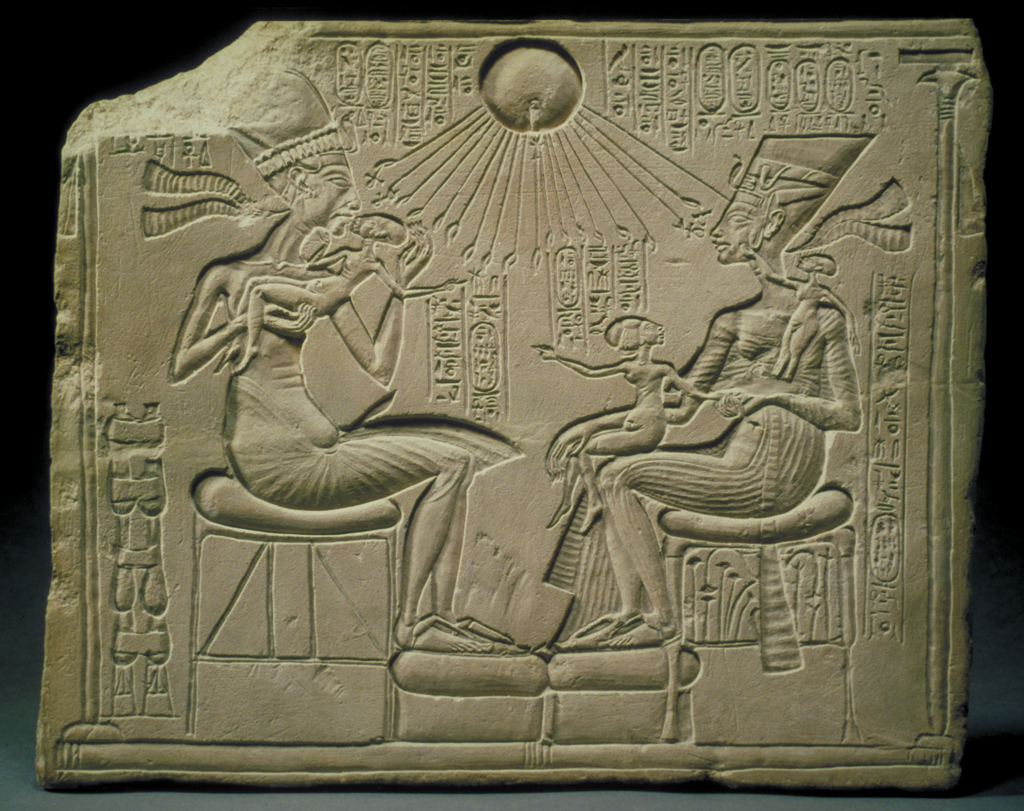
\includegraphics[width=\textwidth]{aten}
Creative Commons Licence, Minneapolis College of Art and Design \\
Attribution 2.0 Generic (CC BY 2.0)
\end{center}
\newpage
\begin{center}
\tableofcontents
\end{center}
\section{Introduction}
While we cannot draw a flag variety, or even its associated root system (except in low dimensions), we can always draw its Hasse diagram.
Our eyes immediately spot in that Hasse diagram its uppermost component, which is always the Hasse diagram of a unique cominuscule variety.
We then predict (correctly, as we will see) that each flag variety contains an associated homogeneous cominuscule subvariety, whose root system is a subsystem of the root system of the flag variety.
Flag varieties have few regular maps between them \cite{bakshi2023morphisms,kumar2023nonexistence,naldi2022morphisms,occhetta2023morphisms,Sierra:2021,Tango:1974,Tango:1976}, hence few flag subvarieties, so these subvarieties are surprising, and we expect them to be important.
\begin{example}
As in the image of Aten's rays, pick a point \(p_0\) and a line \(\ell_0\) in projective space \(\Proj{2}\), with \(p_0\) not lying on \(\ell_0\).
\[
\begin{tikzpicture}
\clip[rounded corners=10pt] (0,0) -- (4,0) -- (4,2.45) -- (0,2.45) -- cycle;
\node[anchor=south west,inner sep=0] at (0,0) {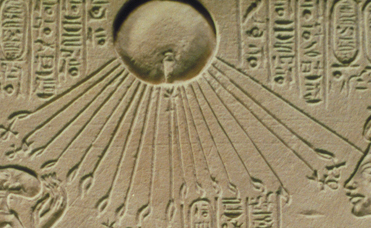
\includegraphics[width=4cm]{aten-crop.jpg}};
\def\x{1.8}
\def\y{2.225}
    \coordinate (sun) at (\x,\y) {};
    \fill[black] (sun) circle (2pt);
%\def\r{.15}
%\def\R{4}
%\begin{scope}
%\clip (0,.75) rectangle (4,2.5);
%   \foreach \i in {7,...,29}
%{
%\draw[rounded corners,white] ({\x+\r*cos(180+5*\i)},{\y+\r*sin(180+5*\i)}) -- ++({\R*cos(180+5*\i)},{\R*sin(180+5*\i)});
%}
%\end{scope}
    \draw[black,ultra thick,rounded corners] (0,.75) -- (4,.75);
\end{tikzpicture}
\]
Each point \(p\) of \(\ell_0\) has an associated pointed line: the pair \((p,pp_0)\).
\[
\begin{tikzpicture}
\clip[rounded corners=10pt] (0,0) -- (4,0) -- (4,2.45) -- (0,2.45) -- cycle;
\node[anchor=south west,inner sep=0] at (0,0) {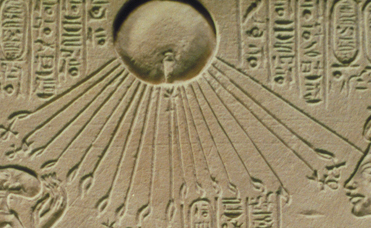
\includegraphics[width=4cm]{aten-crop.jpg}};
\def\x{1.8}
\def\y{2.225}
    \coordinate (sun) at (\x,\y) {};
    \fill[black] (sun) circle (2pt);
\def\r{.15}
\def\R{4}
\begin{scope}
\clip (0,.75) rectangle (4,2.5);
   \foreach \i in {7,...,29}
{
\draw[white,opacity=.5,thick] ({\x+\r*cos(180+5*\i)},{\y+\r*sin(180+5*\i)}) -- ++({\R*cos(180+5*\i)},{\R*sin(180+5*\i)});
}
\end{scope}
    \draw[black,ultra thick,rounded corners] (0,.75) -- (4,.75);
\end{tikzpicture}
\]
These pointed lines form a rational curve in the variety of pointed lines (\emph{not} in \(\Proj{2}\)). 
This rational curve is homogeneous under the projective transformations fixing \(p_0\) and \(\ell_0\); it is the associated cominuscule variety to the variety of pointed lines.
Each Cartan subgroup of the projective transformations of the plane consists of those which preserve three points in general position:
\[
\begin{tikzpicture}
\clip[rounded corners=10pt] (0,0) -- (4,0) -- (4,2.45) -- (0,2.45) -- cycle;
\node[anchor=south west,inner sep=0] at (0,0) {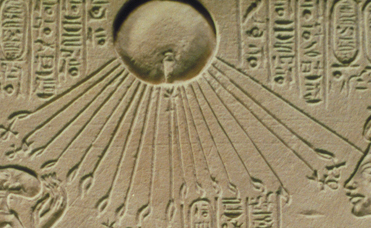
\includegraphics[width=4cm]{aten-crop.jpg}};
\def\x{1.8}
\def\y{2.225}
    \coordinate (sun) at (\x,\y) {};
    \fill[thick,black,draw=white] (sun) circle (2pt);
\def\r{.15}
\def\R{4}
%\begin{scope}
%\clip (0,.75) rectangle (4,2.5);
%   \foreach \i in {7,...,29}
%{
%\draw[rounded corners,white] ({\x+\r*cos(180+5*\i)},{\y+\r*sin(180+5*\i)}) -- ++({\R*cos(180+5*\i)},{\R*sin(180+5*\i)});
%}
%\end{scope}
    \draw[black,ultra thick,rounded corners] (0,.75) -- (4,.75);
    \fill[thick,black,draw=white] (.35,.75) circle (2pt);
    \fill[thick,black,draw=white] (3.5,.75) circle (2pt);
\end{tikzpicture}
\]
Hence the associated cominiscule is invariant under a Cartan subgroup, and conversely there are finitely many associated cominiscules invariant under any given Cartan subgroup.
The projective transformations preserving the point \(p_0\) and line \(\ell_0\) act transitively on the associated cominiscule, moving the points \(p\) of the line \(\ell_0\).
\end{example}
\begin{example}\label{example:flag}
Take a vector space \(V\) and write it as the direct sum of linear subspaces \(V_i\subseteq V\), say of dimension \(n_i\), \(i=1,2,\dots,k\).
Let \(G\defeq\SL{V}\).
Let \(P\subset G\) be the subgroup of linear transformations preserving the successive sums 
\[
V_1,V_1\oplus V_2,\dots,V_1\oplus\dots\oplus V_k=V.
\]
So \(X:=G/P\) is the set of partial flags of dimensions 
\[
0,n_1,n_1+n_2,\dots,n_1+\dots+n_k=n.
\]
Let \(\breve{G}\subset G\) be the subgroup preserving \(V_1\oplus V_k\) and acting as the identity on every \(V_i\), \(i=2,\dots,k-1\).
Let \(\breve{P}\subseteq\breve{G}\) be the subgroup preserving \(V_1\).
Then every element of \(\breve{P}\) preserves \(V_1,V_1\oplus V_2,\dots\), hence \(\breve{P}\subseteq P\).
So \(\breve{X}=\breve{G}/\breve{P}\subseteq X=G/P\) is the Grassmannian inside the partial flag variety \(X\).
The points of \(\breve{X}\) are precisely the partial flags
\[
0=W_0\subset W_1\subset \dots \subset W_k=V
\]
for which 
\[
(V_1\oplus V_k)\cap W_1=W_1, V_2\cap W_1=0,V_3\cap W_1=0,\dots,V_{k-1}\cap W_1=0,
\]
and
\[
V_2\subseteq W_2, V_2\oplus V_3\subseteq W_3, \dots, V_2\oplus\dots V_{k-1}\subseteq W_{k-1},
\]
i.e.
\[
\dim W_1=\dim((V_1\oplus V_k)\cap W_1),
0=\dim (V_2\cap W_1)=\dots=\dim (V_{k-1}\cap W_1),
\] 
and
\[
\dim (V_2\cap W_2)\ge n_2,\dots,
\dim ((V_2\oplus\dots V_{k-1})\cap W_{k-1})\ge n_1+\dots+n_{k-1},
\]
so \(\breve{X}\subseteq X\) is an obvious intersection of Schubert cells.
\end{example}
\subsection{Flag varieties}
A \emph{flag variety} \((X,G)\), also called a \emph{generalized flag variety} or a \emph{rational homogeneous variety}, is a complex projective variety \(X\) acted on transitively and holomorphically by a connected complex semisimple Lie group \(G\) \cite{Knapp:2002} p. 325.
We will need to make use of ineffective flag varieties, i.e. \(G\) might not act faithfully on \(X\).
A Lie group \(G\) acts \emph{almost effectively} on a manifold \(X\) if the elements of \(G\) fixing every point of \(X\) form a finite subgroup. 
It is traditional to denote the stabilizer \(G^{x_0}\) of a point \(x_0 \in X\) as \(P\); the subgroup \(P\subseteq G\) is a connected complex linear algebraic subgroup.
(A subgroup of \(G\) is \emph{parabolic} if it is the stabilizer of a point of a flag variety \((X,G)\) of \(G\), hence the use of the letter \(P\).)

Denote the Lie algebras of \(P\subseteq G\) by \(\LieP\subset\LieG\). 
One can select a Cartan subgroup of \(G\) lying inside \(P\), whose positive root spaces all lie in \(\LieP\).
A simple root \(\aa\) is \(P\)-\emph{compact} (\emph{compact} if \(P\) is understood) if the root space of \(-\aa\) belongs to the Lie algebra of \(P\).
Each flag variety is determined uniquely, up to finite central extension of \(G\) and up to isomorphism, by the Dynkin diagram of \(G\) decorated with \(\dynkin{A}{*}\) on each compact simple root and \(\dynkin{A}{x}\) on each noncompact root \cite{Borel:1991} p. 197 Proposition 14.18.
\subsection{Reducible flag varieties}\label{subsec:reducible}
The center of any complex semisimple Lie group \(G\) lies in every maximal torus, so in every Cartan subgroup \cite{Borel:1991} p. 220, so in every parabolic subgroup, so acts trivially on every flag variety.
An \emph{irreducible} flag variety is a flag variety \((X,G)\) with \(G\) a simple Lie group, and with only the center of \(G\) acting trivially.
Every flag variety \((X,G)\), up to finite central extension of \(G\), admits a factorization 
\begin{align*}
X&=X_0 \times X_1 \times X_2 \times \dots \times X_s, \\
G&=G_0 \times G_1 \times G_2 \times \dots \times G_s, 
\end{align*}
into irreducible flag varieties \(\pr{X_i, G_i}\), \(i>0\), and a point \(X_0=\set{x_0}\), unique up to permutation of the \((X_i,G_i)\) for \(i>0\) and isomorphism.
The flag variety \((X,G)\) is effective if and only if all \((X_i,G_i)\) are effective, i.e. if and only if \(G_0=\set{1}\) is trivial and \(G_1,\dots,G_s\) are in adjoint form.
\subsection{Cominuscule varieties}
A flag variety is \emph{cominuscule} if \(\LieG/\LieP=T_{x_0} X\) is a sum of irreducible complex algebraic \(P\)-modules.
This occurs just when there is a compact subgroup \(K\subseteq G\) so that \(\pr{X,K}\) is a compact Hermitian symmetric space \cite{Kostant:1961} p. 379 Proposition 8.2, \cite{Baston/Eastwood:1989} p. 26.
Some authors prefer the term \emph{compact Hermitian symmetric space}, \emph{cominuscule Grassmannian}, or \emph{generalized Grassmannian} to \emph{cominuscule variety}.
Every effective cominuscule variety is a product of the following irreducible effective cominuscule varieties \cite{Kobayashi/Nagano:1964} theorem 1 p. 401:\par\noindent{}%
%%%\documentclass{amsart}
%\pdfoutput=1
%\usepackage{array}
%\usepackage{longtable}
%\usepackage{xparse}
%\usepackage{colortbl}
%\usepackage{booktabs}
%\usepackage{dynkin-diagrams}
%\NewDocumentCommand\pr{m}{\ensuremath{\left(#1\right)}}
%\NewDocumentCommand\curly{m}{\ensuremath{\left\{#1\right\}}}
%\NewDocumentCommand\of{m}{\ensuremath{\!\pr{#1}}}
%\newcolumntype{C}{>{\columncolor[gray]{.9}}>{$}c<{$}}
%\newcolumntype{L}{>{\columncolor[gray]{.9}}>{$}l<{$}}
%\newcolumntype{R}{>{\columncolor[gray]{.9}}>{$}r<{$}}
%\arrayrulecolor{white}
%\setlength{\arrayrulewidth}{.12em}
%\NewDocumentEnvironment{longtabl}{m}%
%{%
%\renewcommand{\arraystretch}{2}%
%\begin{longtable}{#1}%
%}%
%{%
%\end{longtable}%
%\renewcommand{\arraystretch}{1}%
%}%
%\NewDocumentCommand\C{o}%
%{%
%\IfValueTF{#1}%
%{%
%	\ensuremath{\mathbb{C}^{#1}}%
%}%
%{%
%	\ensuremath{\mathbb{C}}%
%}%
%}%
%\NewDocumentCommand\Proj{m}{\ensuremath{\mathbb{P}^{#1}}}
%\begin{document}
\begingroup
\small
\begin{longtabl}{@{}%
>{\columncolor[gray]{.9}$}r<{$}%
>{\columncolor[gray]{.93}}p{2.6cm}%
>{\columncolor[gray]{.9}$}r<{$}%
>{\columncolor[gray]{.93}}l@{}}
\toprule
G&\(G/P\)&\operatorname{dim}&\text{description}\\
\midrule
\endfirsthead
\toprule
G&\(G/P\)&\operatorname{dim}&\text{description}\\
\midrule
\endhead
\bottomrule
\endfoot
\bottomrule
\endlastfoot
A_r&\dynkin{A}{**.*x*.**}&k(r+1-k)&Grassmannian of $k$-planes in $\C[r+1]$
\\
B_r&\dynkin[parabolic=1]{B}{}&2r-1&quadric hypersurface in $\Proj{2r}$\\
C_r&\dynkin[parabolic=16]{C}{}&\frac{r(r+1)}{2}&space of Lagrangian $r$-planes in $\C[2r]$\\
D_r&\dynkin[parabolic=1]{D}{}&2r-2&quadric hypersurface in $\Proj{2r-1}$\\
D_r&\dynkin[parabolic=32]{D}{}&\frac{r(r-1)}{2}& %one component of the variety of 
space of null $r$-planes in $\C[2r]$ \\
E_6&\dynkin[parabolic=1]{E}{6}&16&complexified octave projective plane\\
E_7 &\dynkin[parabolic=64]{E}{7}&27&space of null octave \(3\)-planes in octave \(6\)-space
\end{longtabl}
\endgroup
%\end{document}
\begingroup
\small
\begin{longtabl}{@{}%
>{\columncolor[gray]{.9}$}r<{$}%
>{\columncolor[gray]{.93}}p{2.6cm}%
>{\columncolor[gray]{.9}$}r<{$}%
>{\columncolor[gray]{.93}}l@{}}
\toprule
G&\(G/P\)&\operatorname{dim}&\text{description}\\
\midrule
\endfirsthead
\toprule
G&\(G/P\)&\operatorname{dim}&\text{description}\\
\midrule
\endhead
\bottomrule
\endfoot
\bottomrule
\endlastfoot
A_r&\dynkin[labels={,,,k,,,}]{A}{**.*x*.**}&k(r+1-k)&Grassmannian of $k$-planes in $\C[r+1]$
\\
B_r&\dynkin[parabolic=1]{B}{}&2r-1&quadric hypersurface in $\Proj{2r}$\\
C_r&\dynkin[parabolic=16]{C}{}&\frac{r(r+1)}{2}&space of Lagrangian $r$-planes in $\C[2r]$\\
D_r&\dynkin[parabolic=1]{D}{}&2r-2&quadric hypersurface in $\Proj{2r-1}$\\
D_r&\dynkin[parabolic=32]{D}{}&\frac{r(r-1)}{2}& %one component of the variety of 
space of null $r$-planes in $\C[2r]$ \\
E_6&\dynkin[parabolic=1]{E}{6}&16&complexified octave projective plane\\
E_7 &\dynkin[parabolic=64]{E}{7}&27&space of null octave \(3\)-planes in octave \(6\)-space
\end{longtabl}
\endgroup
%% end input
\subsection{Structure of linear algebraic groups}
A complex linear map is \emph{unipotent} if its only eigenvalue is \(1\).
A subgroup of a linear algebraic group is \emph{unipotent} if it consists of unipotent linear maps.
Every complex linear algebraic group \(G\) has a \emph{unipotent radical}, the unique maximal unipotent normal subgroup, which is a closed complex linear algebraic subgroup \cite{Borel:1991} p. 85 Theorem 4.5, p. 86 Theorem 4.7, p. 157 11.21.

A complex linear algebraic group is \emph{reductive} if it contains a Zariski dense compact subgroup \cite{Knapp:2002} p. 382 Proposition 7.15.
Every complex linear algebraic group \(G\) has a \emph{reductive Levi factor}, i.e. a maximally reductive complex linear algebraic subgroup,  unique up to conjugacy, so that \(G\) is a semidirect product of its reductive Levi factor and its unipotent radical \cite{Borel:1991} p. 158 11.22.
Any Cartan subgroup is therefore a subgroup of the Levi factor, after perhaps a conjugacy.
Every compact subgroup lies in a maximal compact subgroup, which is unique up to conjugacy, so lies in the Levi factor up to conjugacy \cite{Hilgert.Neeb:2012} p. 531 Theorem 14.1.3.
After perhaps extending by some finite group of order a power of \(2\), the Weyl group embeds in \(G\) as a finite subgroup \cite{Tits:1966}, hence compact, so this group lies in the Levi factor up to conjugacy.

\subsection{Parabolic subgroups}
A Zariski closed subgroup \(P\subseteq G\) of a connected linear algebraic group \(G\) is \emph{parabolic} if \(X:=G/P\) is a projective variety, and this occurs just when \((X,G)\) is a flag variety, and just when \(P\) contains a maximal connected solvable subgroup \cite{Borel:1991} p. 148.
Every parabolic subgroup is connected p. 197 Proposition 14.18.
The unipotent radical of \(P\) is denoted \(\GN\subseteq P\), and a maximal reductive Levi factor is denoted \(\GZ\subseteq P\), so \(P=\GZ\ltimes\GN\).
(This is potentially confusing; the reader might expect to write these as \(P_+\) and \(P_0\) since they lie in \(P\), but this notation is standard \cite{Cap/Slovak:2009} p. 293 theorem 3.2.1, and due to the presence of the grading of the Lie algebra of \(G\) which we will define.)
A flag variety is cominuscule just when \(\GN\) is abelian \cite{Cap/Slovak:2009} p. 296 \S{}3.2.3.
Denote the center of the unipotent radical by \(Z\defeq Z_{\GN}\).
\subsection{Opposite parabolic subgroups}
All Borel subgroups of \(G\) are conjugate \cite{Borel:1991} p. 147 chapter IV 11.1, each containing a Cartan subgroup, hence the Lie algebra of \(P\) is a sum of root spaces with the Cartan subalgebra.
Every automorphism of a root system arises from an automorphism of the associated semisimple Lie group.
Hence there is an automorphism \(G\xrightarrow{a}G\) of \(G\) which yields \(\alpha\mapsto-\alpha\) in the root system.
(We can define such an automorphism explicitly as \(e_{\alpha}\mapsto -e_{-\alpha}\) on root vectors in a Chevalley basis; see section~\vref{subsubsection:ChevalleyBases}.)
Our automorphism sends \(P\) to its \emph{opposite} \(aP\) parabolic subgroup, so gives \(P\cap aP=\GZ\) and \(G_+\cap aG_+=\set{1}\) and an open subset of \(G\) consists of elements uniquely expressed as a product \(p,q\in P\times aG_+\mapsto pq\in G\) \cite{Cap/Slovak:2009} p. 294, \cite{Borel:1991} p. 198 Proposition 14.21.
\subsection{Definition of the associated cominiscule}
Let \(\breve{G}\defeq\left<Z,aZ\right> \subseteq G\) be the subgroup generated by \(Z\cup aZ\), \(\breve{P} \defeq \breve{G} \cap P\), \(\breve{X} \defeq \breve{G}/\breve{P}\).
Then \((\breve{X},\breve{G})\) is the \emph{associated cominuscule subvariety} through the point \(x_0\in X\).
\subsection{Example: the general linear flag variety}
We return to the study of the flag varieties of \(A_{n-1}=\PSL{n}\); see example~\vref{example:flag}.
We took a vector space \(V\) of dimension \(n\).
We let \(G\defeq\PSL{V}\) and \(X\) the set of partial flags of dimensions 
\[
0,n_1,n_1+n_2,\dots,n_1+\dots+n_k=n.
\]
We wrote \(V\) as the direct sum of linear subspaces \(V_i\subseteq V\), say of dimension \(n_i\), \(i=1,2,\dots,k\).
Supposing that \(V=\C[n]\), our automorphism becomes transpose inverse.
To be explicit, for simplicity we suppose \(k=4\).
In our table, each line is a pair \(\Gamma \ M\), 
of a group \(\Gamma\) and a matrix \(M\) with some unspecified entries, to mean that \(\Gamma\) is the group of unimodular matrices of the given form \(M\), modulo rescaling by the matrices \(\lambda I\) of that form where \(\lambda\) is an \(n^{\textnormal{th}}\) root of unity.
\begin{longtable}{@{}>{$\mathrlap}c<{$}>{$}c<{$}@{}}
G&\begin{pmatrix}
*&*&*&*\\
*&*&*&*\\
*&*&*&*\\
*&*&*&*
\end{pmatrix}\\[3em]
P&\begin{pmatrix}
*&*&*&*\\
0&*&*&*\\
0&0&*&*\\
0&0&0&*
\end{pmatrix}\\[3em]
G_+&
\begin{pmatrix}
I&*&*&*\\
0&I&*&*\\
0&0&I&*\\
0&0&0&I
\end{pmatrix}\\[3em]
Z&\begin{pmatrix}
I&0&0&*\\
0&I&0&0\\
0&0&I&0\\
0&0&0&I
\end{pmatrix}\\[3em]
G_0&\begin{pmatrix}
*&0&0&0\\
0&*&0&0\\
0&0&*&0\\
0&0&0&*
\end{pmatrix}\\[3em]
\breve{G}&
\begin{pmatrix}
*&0&0&*\\
0&I&0&0\\
0&0&I&0\\
*&0&0&*
\end{pmatrix}\\[3em]
G'&\begin{pmatrix}
*&0&0&*\\
0&*&0&0\\
0&0&*&0\\
*&0&0&*
\end{pmatrix}\\[3em]
P'&
\begin{pmatrix}
*&0&0&*\\
0&*&0&0\\
0&0&*&0\\
0&0&0&*
\end{pmatrix}
\end{longtable}
To be more precise, \(G_+\) consists of the matrices 
\[
\begin{pmatrix}
\lambda I&*&*&*\\
0&\lambda I&*&*\\
0&0&\lambda I&*\\
0&0&0&\lambda I
\end{pmatrix}
\]
with determinant \(1\), up to rescaling by \(n^{\text{th}}\) roots of unity.
But for each such matrix equivalence class, pick any representative and we can pick that root of unity uniquely to write it as an actual matrix with \(\lambda=1\), and similarly for \(Z\).
Clearly \(\breve{G}\) has Lie algebra containing all root vectors of all \(P\)-maximal and \(P\)-minimal roots, and is generated by the \(1\)-parameter subgroups of those root vectors.
So it contains the root vectors of the root system generated by these, and the Cartan subgroup of that root system, hence a semisimple group.
Note that \(P'\) preserves \(V_1\), \(V_2\), \(V_3\), and \(V_1\oplus V_4\), while
\(G'\) preserves \(V_2\), \(V_3\) and \(V_1\oplus V_4\).
So \(\breve{X}=\breve{G}/\breve{P}=G'/P'\) is the Grassmannian of linear subspaces of dimension \(n_1\) inside \(V_1\oplus V_4\).

\subsection{Finding the associated cominiscule subvariety}
We will prove~\vpageref{page:associated.cominuscule}:
\begin{lemma}\label{lemma:associated.cominuscule}
The complex homogeneous space \((\breve{X},\breve{G})\) is a positive dimensional homogeneously embedded cominuscule subvariety of \((X,G)\).
If \((X,G)\) is almost effective then so is \((\breve{X},\breve{G})\).
The Dynkin diagram of \((\breve{X},\breve{G})\) has one connected component for each connected component of the Dynkin diagram of \((X,G)\).
\end{lemma}
\subsection{Why the associated cominiscule subvariety matters}
We will see \vpageref{subsection:Freedom} that the associated cominiscule subvariety of an irreducible flag variety \((X,G)\) satisfies an open condition on its tangent spaces, which we call \emph{freedom}.
We will see that the symmetry group of the associated cominiscule subvariety has strictly maximal dimension among symmetry groups of subvarieties of \(X\) with free smooth locus.
We will see that all free smooth subvarieties are homogeneous, evidence for the conjecture that the associated cominiscule subvariety is the unique free smooth subvariety.
\section{Statement of the theorem}
\begin{theorem}
With \(\dynkin{A}{o}\) denoting a node which could be either a \(\dynkin{A}{x}\) or \(\dynkin{A}{*}\), the associated cominuscule subvarieties are:
\end{theorem}
%%%\documentclass{amsart}
%\pdfoutput=1
%\usepackage{lmodern}
%\usepackage{cfr-lm}
%\usepackage[T2A,T1]{fontenc}
%\usepackage[utf8]{inputenx}
%\usepackage{etex}
%\usepackage{mathtext}
%\ifdefined\hypersetup%
%\else%
%\usepackage[pdftex,pagebackref]{hyperref}%
%\fi%
%\hypersetup{
%  colorlinks   = true,  %Colours links instead of ugly boxes
%  urlcolor     = black, %Colour for external hyperlinks
%  linkcolor    = black, %Colour of internal links
%  citecolor    = black  %Colour of citations
%}
%\usepackage[kerning=true,tracking=true]{microtype}
%\usepackage{amsfonts}
%\usepackage{amssymb}
%\usepackage{mathtools}
%\usepackage{mathabx}
%\usepackage{braket}
%\usepackage{cool}
%\usepackage[draft]{varioref}
%\usepackage{array}
%\usepackage{ragged2e}
%\usepackage{longtable}
%\usepackage[longtable]{multirow}
%\usepackage{booktabs}
%\usepackage{enumitem}
%\usepackage{dynkin-diagrams}
%\usepackage{colortbl}
%%% Commands
%\NewDocumentCommand\pr{m}{\ensuremath{\left(#1\right)}}
%\NewDocumentCommand\curly{m}{\ensuremath{\left\{#1\right\}}}
%\NewDocumentCommand\of{m}{\ensuremath{\!\pr{#1}}}
%\RenewDocumentCommand\C{o}%
%{%
%	\ensuremath%
%	{%
%		\IfValueTF{#1}%
%		{%
%			\mathbb{C}^{#1}%
%		}%
%		{%
%			\mathbb{C}%
%		}%
%	}%
%}%
%
%\newcolumntype{C}{>{\columncolor[gray]{.9}}>{$}c<{$}}
%\newcolumntype{L}{>{\columncolor[gray]{.9}}>{$}l<{$}}
%\newcolumntype{R}{>{\columncolor[gray]{.9}}>{$}r<{$}}
%
%\makeatother
%\arrayrulecolor{white}
%\setlength{\arrayrulewidth}{.12em}
%
%\NewDocumentEnvironment{longtabl}{m}%
%{%
%\renewcommand{\arraystretch}{2}%
%\begin{longtable}{#1}%
%}%
%{%
%\end{longtable}%
%\renewcommand{\arraystretch}{1}%
%}%
%\begin{document}
\begingroup
% \LastFlag in each group has to indicate the number of flag varieties in the series, and the name of the series. It is starred if it is the last flag variety in the table.
\NewDocumentCommand\LastFlag{smmmm}%
{%%
	\multirow{-#2}{*}%
		{%
			\(#3\)%
		}%
		\Flag{#4}{#5}%
		\IfBooleanF{#1}{\hline}%
}%%
\NewDocumentCommand\Flag{mm}{&#1&#2\\*}
\begin{longtabl}{@{}R>{\columncolor[gray]{.93}}>{$}r<{$}L@{}}
\toprule
&G/P&\breve{G}/\breve{P}\\
\midrule
\endfirsthead
\multicolumn{3}{c}{\dots continued}\\
\toprule
&G/P&\breve{G}/\breve{P}\\
\midrule
\endhead
\midrule
\multicolumn{2}{c}{continued \dots}\\
\endfoot
\bottomrule
\endlastfoot
\LastFlag{1}{A_r}{%
\begin{dynkinDiagram}{A}{*.*xo.ox*.*} 
\dynkinBrace[p]{1}{2}
\dynkinBrace[q]{7}{8}
\end{dynkinDiagram}%
}{%
\begin{dynkinDiagram}{A}{*.*x*.*} 
\dynkinBrace[p]{1}{2}
\dynkinBrace[q]{4}{5}
\end{dynkinDiagram}%
}%
\Flag{\dynkin[parabolic=1]{B}{}}{\dynkin[parabolic=1]{B}{}}
\Flag{\dynkin{B}{oxo.ooo}}{\dynkin{A}{x}}
\Flag{%
\begin{dynkinDiagram}{B}{x*.*xo.ooo}
\dynkinBrace[\ell\ge 2]{1}{4}
\end{dynkinDiagram}%
}{%
\begin{dynkinDiagram}{A}{x*.*}
\dynkinBrace[\ell]{1}{3}
\end{dynkinDiagram}%
}%
\LastFlag{4}{B_r}{%
\begin{dynkinDiagram}{B}{**.*xo.ooo}
\dynkinBrace[\ell\ge 3]{1}{4}
\end{dynkinDiagram}%
}{%
\begin{dynkinDiagram}{D}{*.**.x}
\dynkinLabelRoot{4}{\ell}
\end{dynkinDiagram}%
}
\Flag{\dynkin[parabolic=16]{C}{}}{\dynkin[parabolic=16]{C}{}}%
\Flag{\dynkin{C}{xo.ooo}}{\dynkin{A}{x}}%
\LastFlag{3}{C_r}{%
\begin{dynkinDiagram}{C}{*.*xo.ooo}
\dynkinBrace[\ell\ge 2]{1}{3}
\end{dynkinDiagram}%
}{%
\begin{dynkinDiagram}[parabolic=16]{C}{}
\dynkinBrace[\ell]{1}{5}
\end{dynkinDiagram}%
}%
\Flag{\dynkin[parabolic=1]{D}{}}{\dynkin[parabolic=1]{D}{}}%
\Flag{\dynkin[parabolic=32]{D}{}}{\dynkin[parabolic=32]{D}{}}%
\Flag{\dynkin[parabolic=16]{D}{}}{\dynkin[parabolic=16]{D}{}}%
\LastFlag{4}{D_r}{%
\begin{dynkinDiagram}{D}{o*.*xo.ooo}
\dynkinBrace[\ell\ge 2]{1}{4}
\end{dynkinDiagram}%
}{%
\begin{dynkinDiagram}[parabolic=1]{A}{}
\dynkinBrace[\ell-1]{1}{4}
\end{dynkinDiagram}%
}%
\Flag{\dynkin[ordering=Carter]E{oooxoo}}{\dynkin A{x}}
\Flag{\dynkin[ordering=Carter]E{oox*oo}}{\dynkin A{x*}}
\Flag{\dynkin[ordering=Carter]E{ox**xo}}{\dynkin A{x**}}
\Flag{\dynkin[ordering=Carter]E{x***xo}}{\dynkin A{x***}}
\Flag{\dynkin[ordering=Carter]E{****xo}}{\dynkin A{x****}}
\Flag{\dynkin[ordering=Carter]E{x****x}}{\dynkin[ordering=Carter]D{x****}}
\LastFlag{7}{E_6}{\dynkin[ordering=Carter]E{x*****}}{\dynkin[ordering=Carter]E{x*****}}
\Flag{\dynkin[ordering=Carter]E{oooooox}}{\dynkin A{x}}
\Flag{\dynkin[ordering=Carter]E{ooooox*}}{\dynkin A{x*}}
\Flag{\dynkin[ordering=Carter]E{oooxo**}}{\dynkin A{x**}}
\Flag{\dynkin[ordering=Carter]E{oox*x**}}{\dynkin A{x***}}
\Flag{\dynkin[ordering=Carter]E{oox****}}{\dynkin A{x****}}
\Flag{\dynkin[ordering=Carter]E{ox**x**}}{\dynkin A{x****}}
\Flag{\dynkin[ordering=Carter]E{x***x**}}{\dynkin A{x*****}}
\Flag{\dynkin[ordering=Carter]E{****x**}}{\dynkin A{x******}}
\Flag{\dynkin[ordering=Carter]E{ox*****}}{\dynkin D{x*****}}
\LastFlag{10}{E_7}{\dynkin[ordering=Carter]E{x******}}{\dynkin[ordering=Carter]E{x******}}
\Flag{\dynkin[ordering=Carter]{E}{xooooooo}}{\dynkin{A}{x}}
\Flag{\dynkin[ordering=Carter]{E}{*xoooooo}}{\dynkin{A}{x*}}
\Flag{\dynkin[ordering=Carter]{E}{**xooooo}}{\dynkin{A}{x**}}
\Flag{\dynkin[ordering=Carter]{E}{***xoooo}}{\dynkin{A}{X***}}
\Flag{\dynkin[ordering=Carter]{E}{****xooo}}{\dynkin{A}{x****}}
\Flag{\dynkin[ordering=Carter]{E}{*****xoo}}{\dynkin{A}{x*****}}
\Flag{\dynkin[ordering=Carter]{E}{******xo}}{\dynkin{A}{x******}}
\LastFlag{8}{E_8}{\dynkin[ordering=Carter]{E}{*******x}}{\dynkin[parabolic=1]{D}{8}}
\Flag{\dynkin[ordering=Carter]F{xooo}}{\dynkin A{x}}
\Flag{\dynkin[ordering=Carter]F{*xoo}}{\dynkin A{x*}}
\Flag{\dynkin[ordering=Carter]F{**xo}}{\dynkin A{x**}}
\LastFlag{4}{F_4}{\dynkin[ordering=Carter]F{***x}}{\dynkin B{x***}}
\Flag{\dynkin[parabolic=1]{G}{2}}{\dynkin[parabolic=1]{A}{1}}%
\Flag{\dynkin[parabolic=2]{G}{2}}{\dynkin[parabolic=2]{A}{2}}%
\LastFlag*{3}{G_2}{\dynkin[parabolic=3]{G}{2}}{\dynkin[parabolic=1]{A}{1}}%
\end{longtabl}
\endgroup
%\end{document}
\begingroup
% \LastFlag in each group has to indicate the number of flag varieties in the series, and the name of the series. It is starred if it is the last flag variety in the table.
\NewDocumentCommand\LastFlag{smmmm}%
{%%
	\multirow{-#2}{*}%
		{%
			\(#3\)%
		}%
		\Flag{#4}{#5}%
		\IfBooleanF{#1}{\hline}%
}%%
\NewDocumentCommand\Flag{mm}{&#1&#2\\*}
\begin{longtabl}{@{}R>{\columncolor[gray]{.93}}>{$}r<{$}L@{}}
\toprule
&G/P&\breve{G}/\breve{P}\\
\midrule
\endfirsthead
\multicolumn{3}{c}{\dots continued}\\
\toprule
&G/P&\breve{G}/\breve{P}\\
\midrule
\endhead
\midrule
\multicolumn{2}{c}{continued \dots}\\
\endfoot
\bottomrule
\endlastfoot
\LastFlag{1}{A_r}{%
\begin{dynkinDiagram}{A}{*.*xo.ox*.*} 
\dynkinBrace[p]{1}{2}
\dynkinBrace[q]{7}{8}
\end{dynkinDiagram}%
}{%
\begin{dynkinDiagram}{A}{*.*x*.*} 
\dynkinBrace[p]{1}{2}
\dynkinBrace[q]{4}{5}
\end{dynkinDiagram}%
}%
\Flag{\dynkin[parabolic=1]{B}{}}{\dynkin[parabolic=1]{B}{}}
\Flag{\dynkin{B}{oxo.ooo}}{\dynkin{A}{x}}
\Flag{%
\begin{dynkinDiagram}{B}{x*.*xo.ooo}
\dynkinBrace[\ell\ge 2]{1}{4}
\end{dynkinDiagram}%
}{%
\begin{dynkinDiagram}{A}{x*.*}
\dynkinBrace[\ell]{1}{3}
\end{dynkinDiagram}%
}%
\LastFlag{4}{B_r}{%
\begin{dynkinDiagram}{B}{**.*xo.ooo}
\dynkinBrace[\ell\ge 3]{1}{4}
\end{dynkinDiagram}%
}{%
\begin{dynkinDiagram}{D}{*.**.x}
\dynkinLabelRoot{4}{\ell}
\end{dynkinDiagram}%
}
\Flag{\dynkin[parabolic=16]{C}{}}{\dynkin[parabolic=16]{C}{}}%
\Flag{\dynkin{C}{xo.ooo}}{\dynkin{A}{x}}%
\LastFlag{3}{C_r}{%
\begin{dynkinDiagram}{C}{*.*xo.ooo}
\dynkinBrace[\ell\ge 2]{1}{3}
\end{dynkinDiagram}%
}{%
\begin{dynkinDiagram}[parabolic=16]{C}{}
\dynkinBrace[\ell]{1}{5}
\end{dynkinDiagram}%
}%
\Flag{\dynkin[parabolic=1]{D}{}}{\dynkin[parabolic=1]{D}{}}%
\Flag{\dynkin[parabolic=32]{D}{}}{\dynkin[parabolic=32]{D}{}}%
\Flag{\dynkin[parabolic=16]{D}{}}{\dynkin[parabolic=16]{D}{}}%
\LastFlag{4}{D_r}{%
\begin{dynkinDiagram}{D}{o*.*xo.ooo}
\dynkinBrace[\ell\ge 2]{1}{4}
\end{dynkinDiagram}%
}{%
\begin{dynkinDiagram}[parabolic=1]{A}{}
\dynkinBrace[\ell-1]{1}{4}
\end{dynkinDiagram}%
}%
\Flag{\dynkin[ordering=Carter]E{oooxoo}}{\dynkin A{x}}
\Flag{\dynkin[ordering=Carter]E{oox*oo}}{\dynkin A{x*}}
\Flag{\dynkin[ordering=Carter]E{ox**xo}}{\dynkin A{x**}}
\Flag{\dynkin[ordering=Carter]E{x***xo}}{\dynkin A{x***}}
\Flag{\dynkin[ordering=Carter]E{****xo}}{\dynkin A{x****}}
\Flag{\dynkin[ordering=Carter]E{x****x}}{\dynkin[ordering=Carter]D{x****}}
\LastFlag{7}{E_6}{\dynkin[ordering=Carter]E{x*****}}{\dynkin[ordering=Carter]E{x*****}}
\Flag{\dynkin[ordering=Carter]E{oooooox}}{\dynkin A{x}}
\Flag{\dynkin[ordering=Carter]E{ooooox*}}{\dynkin A{x*}}
\Flag{\dynkin[ordering=Carter]E{oooxo**}}{\dynkin A{x**}}
\Flag{\dynkin[ordering=Carter]E{oox*x**}}{\dynkin A{x***}}
\Flag{\dynkin[ordering=Carter]E{oox****}}{\dynkin A{x****}}
\Flag{\dynkin[ordering=Carter]E{ox**x**}}{\dynkin A{x****}}
\Flag{\dynkin[ordering=Carter]E{x***x**}}{\dynkin A{x*****}}
\Flag{\dynkin[ordering=Carter]E{****x**}}{\dynkin A{x******}}
\Flag{\dynkin[ordering=Carter]E{ox*****}}{\dynkin D{x*****}}
\LastFlag{10}{E_7}{\dynkin[ordering=Carter]E{x******}}{\dynkin[ordering=Carter]E{x******}}
\Flag{\dynkin[ordering=Carter]{E}{xooooooo}}{\dynkin{A}{x}}
\Flag{\dynkin[ordering=Carter]{E}{*xoooooo}}{\dynkin{A}{x*}}
\Flag{\dynkin[ordering=Carter]{E}{**xooooo}}{\dynkin{A}{x**}}
\Flag{\dynkin[ordering=Carter]{E}{***xoooo}}{\dynkin{A}{X***}}
\Flag{\dynkin[ordering=Carter]{E}{****xooo}}{\dynkin{A}{x****}}
\Flag{\dynkin[ordering=Carter]{E}{*****xoo}}{\dynkin{A}{x*****}}
\Flag{\dynkin[ordering=Carter]{E}{******xo}}{\dynkin{A}{x******}}
\LastFlag{8}{E_8}{\dynkin[ordering=Carter]{E}{*******x}}{\dynkin[parabolic=1]{D}{8}}
\Flag{\dynkin[ordering=Carter]F{xooo}}{\dynkin A{x}}
\Flag{\dynkin[ordering=Carter]F{*xoo}}{\dynkin A{x*}}
\Flag{\dynkin[ordering=Carter]F{**xo}}{\dynkin A{x**}}
\LastFlag{4}{F_4}{\dynkin[ordering=Carter]F{***x}}{\dynkin B{x***}}
\Flag{\dynkin[parabolic=1]{G}{2}}{\dynkin[parabolic=1]{A}{1}}%
\Flag{\dynkin[parabolic=2]{G}{2}}{\dynkin[parabolic=2]{A}{2}}%
\LastFlag*{3}{G_2}{\dynkin[parabolic=3]{G}{2}}{\dynkin[parabolic=1]{A}{1}}%
\end{longtabl}
\endgroup
%% end input
\section{Reducing to root systems}
\subsection{Gradings}
A root system with a basis of simple roots \(\alpha_1,\dots,\alpha_r\) is graded: each root \(\sum n_i \alpha_i\) has grade \(\sum_i n_i\).
For a flag variety \(X=G/P\), the root system is also \emph{\(P\)-graded} by \(\sum n_i\), but summing only over the noncompact simple roots.
The unipotent radical \(G_+\subseteq P\) has Lie algebra the sum of the root vectors of the positively graded roots; clearly this sum is a unipotent Lie algebra, while the zero graded roots are invariant under reflection in one another, giving the semisimple factor of the Levi factor.
A root is \emph{\(P\)-maximal} if it has highest grade in its irreducible factor.
Its root vector then lies inside the center of the unipotent radical of \(P\).
The \emph{box} is the set of \(P\)-maximal roots, terminology which roughly follows \cite{Buch.Chaput.Mihalcea.Perrin:2018}, \cite{Lam.Williams:2008} p. 57, by analogy with Young tableaux.
It is easy to see (see the proof~\vpageref{page:associated.cominuscule} of lemma~\ref{lemma:associated.cominuscule}) that the box generates the root system of \(\breve{G}\).
\subsection{\texorpdfstring{Associated cominuscules in rank \(2\)}{Associated cominuscules in rank 2}}
\begin{example}\label{example:rank.2}
Here we will explain how to read our drawings.
We pick simple roots in our root systems as:
\[
\begin{tikzpicture}[baseline=-.5]
\begin{rootSystem}{A}
\roots
\simpleroots
\end{rootSystem}
\end{tikzpicture} \quad
\begin{tikzpicture}[baseline=-.5]
\begin{rootSystem}{B}
\roots
\simpleroots
\end{rootSystem}
\end{tikzpicture} \quad
\begin{tikzpicture}[baseline=-.5]
\begin{rootSystem}{C}
\roots
\simpleroots
\end{rootSystem}
\end{tikzpicture} \quad
\begin{tikzpicture}[baseline=-.5]
\begin{rootSystem}{G}
\roots
\simpleroots
\end{rootSystem}
\end{tikzpicture}
\]
Start with the roots of \(G_2\):
\[
\begin{tikzpicture}[baseline=-.5]
\begin{rootSystem}{G}
\roots
\end{rootSystem}
\end{tikzpicture}
\]
Each parabolic subgroup has Lie algebra consisting of the sum of the Cartan and the root spaces of those roots which lie on or on one side of a hyperplane, so that the compact roots are those on the hyperplane.
Conversely, draw any hyperplane and it produces a parabolic subgroup.
For example, here is the hyperplane of some parabolic subgroup.
\[
\begin{tikzpicture}[baseline=-.5]
\begin{rootSystem}{G}
\parabolic{2}
\end{rootSystem}
\end{tikzpicture}
\]
Drawing both the hyperplane and roots together:
\[
\begin{tikzpicture}[baseline=-.5]
\begin{rootSystem}{G}
\roots
\parabolic{2}
\end{rootSystem}
\end{tikzpicture}
\]
We can always pick a basis of simple roots so that every simple root lies on the hyperplane (hence a compact simple root) or lies on the chosen side of the hyperplane (a noncompact root):
\[
\begin{tikzpicture}[baseline=-.5]
\begin{rootSystem}{G}
\roots
\parabolic{2}
\simpleroots
\end{rootSystem}
\end{tikzpicture}
\]
(We will instead always pick our hyperplane to allow for the chosen bases of simple roots shown above.)
Grade the roots by height. 
Our hyperplane is always chosen so that we can see the heights, i.e. roots of a given height lie on a parallel hyperplane:
\[
\begin{tikzpicture}[baseline=-.5]
\begin{rootSystem}{G}
\roots
\parabolic{2}
\parabolicgrading
\end{rootSystem}
\end{tikzpicture}
\]
By definition of \(\breve{G}\), its root system is the root system generated by the box, i.e. by the maximal graded roots:
\[
\begin{tikzpicture}[baseline=-.5]
\begin{rootSystem}{G}
\roots
\parabolic{2}
\draw[/root system/grading] (hex cs:x=1,y=1) -- (hex cs:x=2,y=-1);
\end{rootSystem}
\end{tikzpicture}
\]
So the \(\breve{G}\)-roots form the smallest root subsystem containing these.
Finally, draw dark lines through the \(\breve{G}\)-roots:
\[
\begin{tikzpicture}[baseline=-.5]
\begin{rootSystem}{G}
\roots
\parabolic{2}
\draw[/root system/grading] (hex cs:x=-1,y=2) -- (hex cs:x=1,y=1) -- (hex cs:x=2,y=-1) -- (hex cs:x=1,y=-2) -- (hex cs:x=-1,y=-1) -- (hex cs:x=-2,y=1) -- cycle;
\end{rootSystem}
\end{tikzpicture}
\]
The roots of \(\breve{P}=P\cap\breve{G}\) are the roots of \(\breve{G}\) lying on or to the indicated side of the hyperplane: \(4\) of them in our picture.
Hence \(\breve{X}=\breve{G}/\breve{P}\) has dimension equal to the number of roots not lying in \(\breve{P}\), i.e. the dimension of \(\breve{X}\) is the number of roots in the box.
We can see in the picture that the root system of \(\breve{G}\) in this example is that of \(A_2=\PSL{3}\), and that \(\breve{X}\) has dimension \(2\), so must be \((\breve{X},\breve{G})=(\Proj{2},A_2)\).
\end{example}
\begin{example}
We draw the gradings of the positive roots of the parabolic subgroups of the rank \(2\) simple groups.
\begin{longtabl}{@{}>{$\mathrlap}c<{$}ccc@{}}
\toprule
\text{Lie algebra} & \text{Grading} & \text{Associated cominuscule} & \text{Automorphisms}\\ 
\midrule
\endfirsthead
\multicolumn{3}{c}{continued \dots}\\
\toprule
\text{Lie algebra} & \text{Grading} & \text{Associated cominuscule} & \text{Automorphisms}\\ 
\midrule
\endhead
\multicolumn{3}{c}{continued \dots}\\
\endfoot
\bottomrule
\endlastfoot
A_2 & \drawroots{A}{1} 
& 
\begin{tikzpicture}[baseline=-.5]
\begin{rootSystem}{A}
\roots
\parabolic{1}
\draw[/root system/grading] (hex cs:x=-1,y=2) -- (hex cs:x=1,y=1) -- (hex cs:x=2,y=-1) -- (hex cs:x=1,y=-2) -- (hex cs:x=-1,y=-1) -- (hex cs:x=-2,y=1) -- cycle;
\simpleroots
\end{rootSystem}
\end{tikzpicture}
& 
\begin{tikzpicture}[baseline=-.5]
\begin{rootSystem}{A}
\roots
\parabolic{1}
\draw[/root system/grading] (hex cs:x=-1,y=2) -- (hex cs:x=1,y=1) -- (hex cs:x=2,y=-1) -- (hex cs:x=1,y=-2) -- (hex cs:x=-1,y=-1) -- (hex cs:x=-2,y=1) -- cycle;
\simpleroots
\end{rootSystem}
\end{tikzpicture}
 \\ \midrule
A_2 & \drawroots{A}{3} 
& 
\begin{tikzpicture}[baseline=-.5]
\begin{rootSystem}{A}
\roots
\parabolic{3}
\draw[/root system/grading,line width=.3cm] (hex cs:x=1,y=1) -- (hex cs:x=-1,y=-1);
\simpleroots
\end{rootSystem}
\end{tikzpicture}
& 
\begin{tikzpicture}[baseline=-.5]
\begin{rootSystem}{A}
\roots
\parabolic{3}
\draw[/root system/grading,line width=.3cm] (hex cs:x=1,y=1) -- (hex cs:x=-1,y=-1);
\simpleroots
\end{rootSystem}
\end{tikzpicture}
 \\ \midrule
B_2 & \drawroots{B}{1} 
& 
\begin{tikzpicture}[baseline=-.5]
\begin{rootSystem}{B}
\roots
\parabolic{1}
\draw[/root system/grading] (square cs:x=1,y=1) -- (square cs:x=-1,y=1)-- (square cs:x=-1,y=-1)-- (square cs:x=1,y=-1)--cycle;
\simpleroots
\end{rootSystem}
\end{tikzpicture}
& 
\begin{tikzpicture}[baseline=-.5]
\begin{rootSystem}{B}
\roots
\parabolic{1}
\draw[/root system/grading] (square cs:x=1,y=1) -- (square cs:x=-1,y=1)-- (square cs:x=-1,y=-1)-- (square cs:x=1,y=-1)--cycle;
\simpleroots
\end{rootSystem}
\end{tikzpicture}
 \\ \midrule
B_2 & \drawroots{B}{2} 
& 
\begin{tikzpicture}[baseline=-.5]
\begin{rootSystem}{B}
\roots
\parabolic{2}
\draw[/root system/grading,line width=.3cm] (square cs:x=1,y=1) -- (square cs:x=-1,y=-1);
\simpleroots
\end{rootSystem}
\end{tikzpicture}
& 
\begin{tikzpicture}[baseline=-.5]
\begin{rootSystem}{B}
\roots
\parabolic{3}
\draw[/root system/grading,line width=.3cm] (square cs:x=1,y=1) -- (square cs:x=-1,y=-1);
\draw[/root system/grading,line width=.3cm] (square cs:x=-1,y=1) -- (square cs:x=1,y=-1);
\simpleroots
\end{rootSystem}
\end{tikzpicture}
 \\ \midrule
B_2 & \drawroots{B}{3} 
& 
\begin{tikzpicture}[baseline=-.5]
\begin{rootSystem}{B}
\roots
\parabolic{3}
\draw[/root system/grading,line width=.3cm] (square cs:x=1,y=1) -- (square cs:x=-1,y=-1);
\simpleroots
\end{rootSystem}
\end{tikzpicture}
& 
\begin{tikzpicture}[baseline=-.5]
\begin{rootSystem}{B}
\roots
\parabolic{3}
\draw[/root system/grading,line width=.3cm] (square cs:x=1,y=1) -- (square cs:x=-1,y=-1);
\draw[/root system/grading,line width=.3cm] (square cs:x=1,y=-1) -- (square cs:x=0,y=0);
\simpleroots
\end{rootSystem}
\end{tikzpicture}
 \\ \midrule
G_2 & \drawroots{G}{1} 
& 
\begin{tikzpicture}[baseline=-.5]
\begin{rootSystem}{G}
\roots
\parabolic{1}
\draw[/root system/grading,line width=.3cm] (hex cs:x=1,y=1) -- (hex cs:x=-1,y=-1);
\simpleroots
\end{rootSystem}
\end{tikzpicture}
& 
\begin{tikzpicture}[baseline=-.5]
\begin{rootSystem}{G}
\roots
\parabolic{1}
\draw[/root system/grading,line width=.3cm] (hex cs:x=1,y=1) -- (hex cs:x=-1,y=-1);
\draw[/root system/grading,line width=.3cm] (hex cs:x=-1,y=1) -- (hex cs:x=1,y=-1);
\simpleroots
\end{rootSystem}
\end{tikzpicture}
 \\ \midrule
G_2 & \drawroots{G}{2} 
& 
\begin{tikzpicture}[baseline=-.5]
\begin{rootSystem}{G}
\roots
\parabolic{2}
\draw[/root system/grading] (hex cs:x=-1,y=2) -- (hex cs:x=1,y=1) -- (hex cs:x=2,y=-1) -- (hex cs:x=1,y=-2) -- (hex cs:x=-1,y=-1) -- (hex cs:x=-2,y=1) -- cycle;
\simpleroots
\end{rootSystem}
\end{tikzpicture}
& 
\begin{tikzpicture}[baseline=-.5]
\begin{rootSystem}{G}
\roots
\parabolic{2}
\draw[/root system/grading] (hex cs:x=-1,y=2) -- (hex cs:x=1,y=1) -- (hex cs:x=2,y=-1) -- (hex cs:x=1,y=-2) -- (hex cs:x=-1,y=-1) -- (hex cs:x=-2,y=1) -- cycle;
\simpleroots
\end{rootSystem}
\end{tikzpicture}
 \\ \midrule
G_2 & \drawroots{G}{3} 
& 
\begin{tikzpicture}[baseline=-.5]
\begin{rootSystem}{G}
\roots
\parabolic{3}
\draw[/root system/grading,line width=.3cm] (hex cs:x=1,y=1) -- (hex cs:x=-1,y=-1);
\simpleroots
\end{rootSystem}
\end{tikzpicture}
& 
\begin{tikzpicture}[baseline=-.5]
\begin{rootSystem}{G}
\roots
\parabolic{3}
\draw[/root system/grading,line width=.3cm] (hex cs:x=1,y=1) -- (hex cs:x=-1,y=-1);
\draw[/root system/grading,line width=.3cm] (hex cs:x=0,y=0) -- (hex cs:x=1,y=-1);
\simpleroots
\end{rootSystem}
\end{tikzpicture}
\end{longtabl}
\end{example}
\begin{example}
Any maximal irreducible flag variety \(X=G/B\) has associated cominuscule subvariety \(\dynkin[parabolic=1]{A}{1}=(\Proj{1},\PSL{2})\), reducing maximally.
This occurs because \(G\) has a unique highest root, whose root space generates \(Z\).
Similarly, the associated cominiscule of any adjoint variety is \(\dynkin[parabolic=1]{A}{1}=(\Proj{1},\PSL{2})\), since the adjoint varieties are precisely those with invariant contact structures, which arise from a hyperplane in each tangent space, invariant under the parabolic, hence a sum of root spaces, so a single root, negative for the parabolic, doesn't have its root vector in this hyperplane, i.e. a single root is at higher weight.
So the associated cominiscule is complementary to the hyperplane, one dimensional, hence a projective line.
\end{example}
\section{The associated cominuscule is cominuscule}\label{subsection:associated.cominuscule}
Henceforth suppose that \(G\) is a connected complex semisimple Lie group.
\begin{lemma}\label{lemma:breve.G.connected}
The group \(\breve{G}\) is connected.
\end{lemma}
\begin{proof}
Every parabolic subgroup of a connected reductive Lie group is connected, so \(G\) and \(P\) are connected.
By Langlands decomposition \cite{Knapp:2002} p. 482,  \(G,P,X,G_+,G_0\) are connected.
The subgroup \(Z=Z_{G_+}\) is a Zariski closed subgroup of a unipotent linear algebraic group, so connected and isomorphic as an affine variety to complex Euclidean space \cite{Kambayashi/Miyanishi/Takeuchi:1974} p. 147 Remark A.3, \cite{Springer:2009} p. 243 corollary 14.2.7.
Explicitly calculating out that each element
\[
g=e^{\sum t_{\alpha} e_{\alpha}}\in G_+
\]
acts on an element \(e_{\beta}\in G_+\) by
\[
\Ad_g e_{\beta}
\]
expanding out into a sum with entirely positive coefficients unless \(\log g\) is a sum of \(P\)-maximal roots, so the center \(Z=Z_{G_+}\) of \(G_+\) consists precisely of the exponentials of elements of
\[
\LieZ=\bigoplus\LieG_{\alpha},
\]
the sum being over the box, i.e. over the \(P\)-maximal roots, so \(Z\) is connected.
By definition of \(\breve{G}\), \(\breve{G}:=\left<Z,aZ\right>\) is connected, since \(Z\) is connected. 
\end{proof}
%\begin{lemma}
%Two associated cominiscule subvarieties are tangent at a point just when they are equal.
%\end{lemma}
%\begin{proof}
%Suppose that \(T_{x_0}\breve{X}=T_{x_0}g\breve{X}\).
%We can replace \(g\) by \(gh\) for any element \(h\in\breve{G}\), and \(\breve{G}\) acts transitively on \(\breve{X}\) by definition of \(\breve{X}\), so we can arrange that \(gx_0=x_0\), i.e. write \(g\) as \(p\) and we can assume that \(p\in P\).
%These tangent spaces are
%\[
%\breve\LieG/\breve\LieP=\Ad_p\left(\breve\LieG/\breve\LieP\right)\subseteq\LieG/\LieP.
%\]
%So
%\[
%\breve\LieG=\Ad_p\breve\LieG\subseteq\LieG.
%\]
%Hence taking exponentials, the identity components match:
%\[
%\breve{G}=\Ad_p\breve{G}.
%\]
%So their orbits are the same.
%\end{proof}
We prove lemma~\vref{lemma:associated.cominuscule}.
\begin{proof}\label{page:associated.cominuscule}
Take notation as above for a flag variety \(X=G/P\).
It suffices to assume that \((X,G)\) is effective.
It also suffices to assume that \((X,G)\) is an irreducible flag variety, as otherwise it is a product of irreducibles and the subgroup \(\breve{G}\) is the product of the associated subgroups, and so on.
The Lie algebra \(\LieZ\) of the center \(Z\) of the unipotent radical of \(P\) is the sum of the root spaces of the box, i.e. of the \(P\)-maximal roots.
Let \(a\) be the automorphism of \(G\) which changes the sign of the \(P\)-grading of the roots.
So \(a\LieZ\) is the sum of the root spaces of the roots of minimal \(P\)-grade, the opposite box.
Under bracket, these root spaces generate only root vectors and coroots, up to scaling, so the Lie algebra \(\breve\LieG\) of \(\breve{G}\) is the sum of some such, with a coroot only arising when we bracket the root vectors of the associated root and its negative. 
So \(\breve\LieG\) contains all of the root vectors of the root system generated by the box, and their brackets, so contains the complex semisimple subalgebra with that root system.
That subalgebra is generated in the same way, by the box root vectors, so \(\breve\LieG\) is that subalgebra, so is complex semisimple.
By lemma~\vref{lemma:breve.G.connected},  \(\breve{G}\) is a complex semisimple Lie group.
Since its root system lies inside that of \(G\), its Cartan subgroup is a subgroup of the Cartan subgroup of \(G\), generated by its coroots.
Note that \(P\) contains the Cartan subgroup of \(G\), hence that of \(\breve{G}\), and contains \(Z\), so contains the parabolic subgroup of \(\breve{G}\) generated by the box.
So this parabolic subgroup fixes the same point \(x_0\in X\) so lies in \(\breve{P}\).
The \(\breve{G}\)-orbit \(\breve{X}\) of that point \(x_0\) is a flag variety \((\breve{X},\breve{G})\), with stabilizer \(\breve{P}=P\cap\breve{G}\) a parabolic subgroup, so connected.

Since \(\breve\LieG\) is a complex subgroup of \(\LieG\), \(\breve{G}\) is a complex subgroup of \(G\), and so \(\breve{X}\subseteq X\) is a compact complex submanifold, and \(X\) is a smooth projective variety, so \(\breve{X}\subseteq X\) is a smooth subvariety.

The vector spaces \(\LieZ\) and \(a\LieZ\) are irreducible \(\GZ\)-modules \cite{Knapp:2002} p. 332 proposition 5.105.
Hence \(\breve\LieG\) is a \(\GZ\)-module.
As \(\GZ\) is reductive, \(\breve\LieG\) is a direct sum of irreducible \(\GZ\)-modules.

Suppose that \(\aa\) is a \(P\)-compact root which is not a difference of \(P\)-maximal roots.
As \(\aa\) is \(P\)-compact, i.e. a root of \(\GZ\), reflection in \(\aa\) is carried out by an element of the Weyl group of \(\GZ\), and so preserves the \(P\)-grading.
So if \(\bb\) is any \(P\)-maximal root, then so is its \(\aa\)-reflection.
Reflection in \(\aa\) moves \(\bb\) along an \(\aa\)-root string.
If that root string has more than one root in it, then \(\aa\) is a difference of \(P\)-maximal roots.
So reflection in \(\aa\) fixes all \(P\)-maximal roots, and so \(\aa\) is perpendicular to all them.
Reflection in \(\aa\) therefore fixes every root in the root system \(\breve\Roots\) generated by the \(P\)-maximal roots, and therefore is perpendicular to every root in \(\breve\Roots\).
Hence the \(P\)-compact roots divide into (1) those which are differences of \(P\)-maximal roots, i.e. \(\breve{P}\)-compact roots and (2) those perpendicular to \(\breve\Roots\), forming a root subsystem of the \(P\)-compact roots giving a complex semisimple subgroup of \(\GZ\) acting trivially on \(\breve\LieG\).
The root system \(\breve\Roots\) is graded into the \(P\)-minimal roots (grade \(-1\)), differences of \(P\)-maximal roots (grade \(0\)) and \(P\)-maximal roots (grade \(1\)).
The Lie algebra \(\breve\LieG\) consists of the sum of the root vectors of the \(\breve\Roots\)-spaces, and their coroots (grade \(0\)).
The subalgebra \(\breve\LieP\defeq\LieP\cap\breve\LieG\) consists precisely of the \(0\) and \(1\) grades.
Note that \(\breve\LieP\) acts on \(\LieZ\) as \(\breveLieGZ\defeq\LieGZ \cap \breve\LieG\), i.e. as a sum of irreducible \(\breve\LieP\)-modules, so \(\breve{X}=\breve{G}/\breve{P}\) is cominuscule.

Since \(\LieZ\) is an irreducible \(\GZ\)-module, if we start at the highest root, say \(\aa_0\), we can pass from it via root strings to get to any \(P\)-maximal root, i.e. anywhere in the box, repeatedly passing between \(P\)-maximal roots \(\aa,\bb\) by subtracting a \(\breve{P}\)-compact positive root \(\aa-\bb\), so that bracketing a root vector \(\XX{\aa-\bb}\) of root \(\aa-\bb\) takes \(\XX{\aa}\) to a nonzero multiple of \(\XX{\bb}\).
Hence \(\LieZ\) is an irreducible \(\breveLieGZ\)-module, hence an irreducible \(\breve\LieP\)-module.
As we have seen~\vpageref{subsec:reducible}, the number of irreducible modules of the parabolic subgroup is the number of irreducible factors of the flag variety, so \(\breve{X}\) is an irreducible flag variety.

We next prove that \((\breve{X},\breve{G})\) is effective.
An element \(g \in \breve{G}\) acts trivially on \(\breve{X}\) just when \(gg_1\breve{P}=g_1\breve{P}\) for all \(g_1 \in \breve{G}\), i.e. just when \(g\) lies in all \(\breve{G}\)-conjugates of \(\breve{P}\).

The Weyl group acts transitively on bases of simple roots \cite{Serre:2001} p.33 theorem 2.
So we can reverse basis by conjugation by some element of \(G\).
Since \(\breve{P} \subset \breve{G}\) is a parabolic subgroup, conjugation on \(\breve{P}\) and \(P\) reverses the box and its opposite.
But \(\breve{G}_+ \cap a \breve{G}_+=1\) and \(a\breve{G}_0=\breve{G}_+\).
So an element \(g\in\breve{G}\) acting trivially on \(\breve{X}\) lies in \(\breve{G}_0\), the maximal reductive subgroup of \(\breve{P}\).
Acting trivially on \(T_{x_0}\breve{X}\), \(g\) acts trivially on \(\LieZ\).
Reversing, it acts trivially on \(\LieZ_-\), so acts trivially on \(\breve\LieG\), so lies in the center of \(\breve{G}\).
The center lies in the Cartan subgroup, hence in the Cartan subgroup of \(G\).
\end{proof}
\subsection{Automorphisms of the associated cominiscule}
\begin{example}
The flag variety \((X,G)=(B_2/P,B_2)\), where \(P\subseteq B_2\) is the Borel subgroup:
\[
\drawroots{B}{3} 
\]
has associated cominiscule
\[
\begin{tikzpicture}[baseline=-.5]
\begin{rootSystem}{B}
\roots
\parabolic{3}
\draw[/root system/grading,line width=.3cm] (square cs:x=1,y=1) -- (square cs:x=-1,y=-1);
\end{rootSystem}
\end{tikzpicture}
\]
a rational curve \((\breve{X},\breve{G})=(\Proj{1},\PSL{2})\), invariant under not only its automorphism group \(\breve{G}=A_1=\PSL{2}\), which we see in our diagram, but also, as we will see, under rescaling by this root:
\[
\begin{tikzpicture}[baseline=-.5]
\begin{rootSystem}{B}
\roots
\parabolic{3}
\draw[/root system/grading,line width=.3cm] (square cs:x=1,y=1) -- (square cs:x=-1,y=-1);
%\draw (square cs:x=-1,y=1) circle (2pt);
\draw[latex-,shorten <=1mm] (square cs:x=1,y=-1) --++ (.3cm,-.3cm);
\end{rootSystem}
\end{tikzpicture}
\]
The root is perpendicular to the \(\breve{G}\) root system, so commutes with the \(\breve{G}\) root vectors.
The vector field on \(X\) associated to the root vector of that root vanishes at our chosen point \(x_0\in X\) stabilized by \(P\), since the root lies in the Lie algebra of \(P\).
Since the vector field commutes with those of \(\breve{G}\), it is \(\breve{G}\)-invariant.
Since \(\breve{G}\) acts transitively on \(\breve{X}\), our vector field vanishes at all points of \(\breve{X}\).
Hence, in this example, the automorphism group \(G_{\breve{X}}\) of \(\breve{X}\) as a subvariety of \(X\) is larger than the automorphism group \(\breve{G}\) as a flag variety, containing the exponential of this root.

On the other hand, consider the root
\[
\begin{tikzpicture}[baseline=-.5]
\begin{rootSystem}{B}
\roots
\parabolic{3}
\draw[/root system/grading,line width=.3cm] (square cs:x=1,y=1) -- (square cs:x=-1,y=-1);
%\draw (square cs:x=1,y=-1) circle (2pt);
\draw[latex-,shorten <=1mm] (square cs:x=-1,y=1) --++ (-.3cm,.3cm);
\end{rootSystem}
\end{tikzpicture}
\]
It doesn't belong to the Lie algebra of \(P\), so doesn't vanish at \(x_0\).
Commuting with the root vectors of \(\breve{G}\), it is \(\breve{G}\)-invariant, so it doesn't vanish at any point of \(\breve{X}\).
If tangent to \(\breve{X}\) at some point of \(\breve{X}\), and commuting with the root vectors of \(\breve{G}\), it is tangent at every point, nowhere vanishing, not possible on the projective line \(\breve{X}=\Proj{1}\).
Hence this root vector is a vector field on \(X\), nowhere tangent to \(\breve{X}\).
\end{example}
\subsection{Computing the automorphism Lie algebra}
We return our thoughts to the general flag variety \((X,G)\).
By definition of \((\breve{X},\breve{G})\), \(\breve{X}\subset X\) is a smooth subvariety.
So the subgroup \(G'\subseteq G\) leaving \(\breve{X}\subseteq X\) invariant is a Zariski closed subgroup of \(G\), hence linear algebraic.
(As we have noted, we will find that, while \(G'\) contains \(\breve{G}\), it is often larger than \(\breve{G}\) and is not always semisimple.)
Let \(P':=G'\cap P\), so
\[
\breve{X}=\breve{G}/\breve{P}=G'/P'.
\]
Clearly \(\breve{X},\breve{P},\breve{G}\) are connected, so \(G'\) is connected just when \(P'\) is connected.
\begin{theorem}\label{theorem:aut.Lie.alg}
The automorphism group \(G'\) of the associated cominiscule subvariety \(\breve{X}\subset X\) of a flag variety is a complex linear algebraic group with Lie algebra precisely the sum of 
\begin{itemize}
\item
the \(P\)-maximal and \(P\)-minimal root spaces, 
\item
the maximal reductive \(\LieG_0\), and 
\item
the roots spaces of all positive roots perpendicular to all \(P\)-maximal roots.
\end{itemize}
\end{theorem}
\begin{proof}
Clearly \(G'\subseteq G\) is a complex linear algebraic subgroup containing \(\breve{G}\), hence acts transitively on \(\breve{X}\).
Let \(G'_0\subset G'\) be the connected component of the identity.
Since \(\breve{X}\) is connected and \(G'_0\) is a connected linear algebraic group acting transitively on \(\breve{X}\), the stabilizer \(P'_0:=P'\cap G'_0\) of the point \(x_0\in X\) is a parabolic subgroup of \(G'_0\) \cite{Borel:1991} p. 148, hence is connected.
Since \(\breve{X}=G'/P'\) is connected, \(P'\) intersects every component of \(G'\).

Since \(\breve{G}\) acts transitively on \(\breve{X}\), every element of \(G'\) is a product of an element of \(\breve{G}\) and an element of \(P\).
Clearly \(P'\) is the normalizer of \(\breve{G}P\) in \(P\).
Thus \(P'\) contains all elements of \(P\) which normalize \(\breve{G}\).
It contains \(\breve{P}\) and hence contains \(Z=Z_{G_+}\subseteq\breve{P}\).
The maximal reductive \(G_0\subseteq P\) normalizes \(P\) hence \(G_+\) hence \(Z\), and is invariant under the automorphism \(a\).
Thus \(G_0\subseteq P'\).
Hence \(P'\) contains the Cartan subgroup, so its Lie algebra is a sum of the Cartan subalgebra together with various root spaces.

By definition \(P'\) preserves \(\breve\LieG+\LieP\).
Since \(\breve{G},P\) are connected, so is \(\breve{G}P\), and so \(P'\) is precisely the subgroup of \(P\) preserving \(\breve\LieG+\LieP\subseteq\LieG\).
Take a \(P\)-submaximal \(P\)-positive root \(\aa\) at less than right angle with some \(P\)-maximal root \(\mx\bb\).
Then the root vectors of \(\aa\) and \(\mn\bb:=-\mx\bb\) bracket out of \(\breve\LieG+\LieP\).
Hence the Lie algebra \(\LieG'\) of \(G'\) contains no such.

The \(P\)-submaximal \(P\)-positive roots \(\aa\) at a right angle to all \(P\)-maximal roots \(\mx\bb\) have roots vectors commuting, so the root vectors of \(\aa\) preserve \(\breve\LieG\oplus\LieP\).
Roots which are \(P\)-positive are also positive, and conversely if they are not \(P\)-compact.
So \(\LieP'\) contains the root vectors of precisely the \(P\)-maximal roots and the \(P\)-positive roots perpendicular to them, and so consists precisely of these root vectors and the Cartan subalgebra.

The roots whose root vectors lie in \(G'\) contain those of \(P'\): the \(P\)-maximal ones and the \(P\)-positive roots perpendicular to them; and these roots are among the \(P\)-maximal and their perpendiculars.
We have only to check that every \(P\)-negative root \(\aa\) perpendicular to the \(P\)-maximal roots does not have its root vector in \(\LieG'\).
Since \(\aa\) is \(P\)-negative, its associated root vector has associated vector field on \(X\) not vanishing at our chosen point \(x_0\in X\).
Commuting with the root vectors of \(\breve{G}\), it is \(\breve{G}\)-invariant, so it doesn't vanish at any point of \(\breve{X}\).
If tangent to \(\breve{X}\) at some point of \(\breve{X}\), and commuting with the root vectors of \(\breve{G}\), it is tangent at every point, nowhere vanishing, not possible on \(\breve{X}\) since it is a flag variety by lemma~\vref{lemma:associated.cominuscule}.
Hence this root vector is a vector field on \(X\), nowhere tangent to \(\breve{X}\).
\end{proof}

\begin{lemma}
For any flag variety \((X,G)\), the group \(G'\) of automorphisms of the associated cominiscule subvariety \(\breve{X}\subseteq X\) is connected.
The subgroup \(P'\subseteq G'\) fixing a point of \(\breve{X}\) is a connected parabolic subgroup.
\end{lemma}
\begin{proof}
Since \(\breve{G}\subseteq G'\), \(G'\) acts transitively on the connected variety \(\breve{X}\).
We saw in the proof of theorem~\vref{theorem:aut.Lie.alg} that the stabilizer \(P'\subset G'\) of any point \(x_0\in\breve{X}\) intersects every component of \(G'\).
It suffices to prove that \(P'\) is connected.
The subgroup \(G_+':=G_+\cap P'\subset G'\) is unipotent, so connected and isomorphic as an affine variety to complex Euclidean space \cite{Kambayashi/Miyanishi/Takeuchi:1974} p. 147 Remark A.3, \cite{Springer:2009} p. 243 corollary 14.2.7.
But \(G_0\subseteq P'\), so \(P'=G_0\ltimes G_+'\), so is connected.
In the proof of theorem~\vref{theorem:aut.Lie.alg}, we saw that \(P'\) is therefore a parabolic subgroup.
\end{proof}

\begin{theorem}
For any flag variety \((X,G)\), the group \(G'\) of automorphisms of the associated cominiscule subvariety \(\breve{X}\subseteq X\) acts on \(\breve{X}\) as precisely the biholomorphisms of \(\breve{X}\) arising from elements of \(\breve{G}\).
\end{theorem}
\begin{proof}
We can assume that \(G\) acts almost effectively on \(X\).
The automorphism group \(G'\) contains \(\breve{G}\), so its image in the biholomorphisms of \(\breve{X}\) contains the image of \(\breve{G}\), which is a quotient \(\breve{G}/\Gamma\) by a finite subgroup \(\Gamma\subset \breve{G}_0\) of the Levi factor \(\breve{G}_0\subseteq\breve{P}\), central in \(G\).
The Lie algebra \(\LieG'\) maps to the vector fields on \(\breve{X}\), with kernel containing all root spaces of roots perpendicular to the box.
If \((X,G)\) is almost effective, then \(\LieG_0\) acts on \(\breve{\LieG}/\breve{\LieP}=T_{x_0} \breve{X}\) as a sum of irreducibles, each simple factor acting in an irreducible representation, so \(G_0\) acts almost effectively.
Hence \(\LieG'\) mapsto \(\breve\LieG\), an isomorphism on \(\breve\LieG\subseteq\LieG'\).
Since \(G'\) is connected, this map has connected image.
\end{proof}

\section{Hasse diagrams}
\subsection{The Hasse diagram of a root system}
Recall the \emph{Hasse diagram} of a root system.
Given an irreducible reduced root system with a choice of basis of simple roots, and some ordering of the simple roots, a \emph{successor} of a positive root \(\alpha\) is a positive root of the form \(\alpha+\beta\) for a positive simple root \(\beta\).
The \emph{Hasse diagram} draws dots on the plane, one for each positive root, with roots of the same grade on a horizontal line, and a line from each root to each of its successors, labelled by the number of the simple root by which they differ.
(We note that our Hasse diagrams in this paper are drawn by orthogonal linear projection from the dual of the Cartan subalgebra to the plane; this is not required of a Hasse diagram.)
For example, the Hasse diagram of \(F_4\) is
\hasseDiagrams{F4}
\tikzset{/Lie Hasse diagram,attach Dynkin diagram=true,three D=true}
The Hasse diagrams are
\begin{enumerate}
\item[\(A_r\)] Write the simple roots of \(A_r\) as \(\alpha_1,\alpha_2,\dots,\alpha_r\).
Each positive root is a sum of a positive number of \emph{successive} simple roots: \(\alpha_i+\alpha_{i+1}+\dots+\alpha_{i+g-1}\).
This positive root is drawn in the Hasse diagram as a point in the plane, with usual \((x,y)\) Cartesian coordinates: the point \((x,y)=(2i+g,g)\). 
An edge labelled \(i-1\) goes up to the left, if \(i>1\).
An edge labelled \(i+g\) goes up to the right, if \(i+g<r\).
\hasseDiagrams{A5}
\item[\(B_r\)] The union of an \(A_r\) Hasse diagram and its reflection along the upper right side.
\hasseDiagrams{B5}
\item[\(C_r\)] The same as the \(B_r\), but all rightward edge labels in the upper copy of \(A_r\) diminished by one.
\hasseDiagrams{C5}
\item[\(D_r\)] 
Take two \(A_{r-1}\) Hasse diagrams, with one reflected as above, but instead of gluing together, for each matching pair of vertices along the two edges, add a pair of points, connecting one vertex to each with an edge labelled \(r-1\) and an edge labelled \(r\), to make a square with opposite sides having the same label.
\hasseDiagrams{[three D=true]D7}
\end{enumerate}
We draw the Hasse diagrams of all of the exceptional Lie algebras in table~\vref{table:exceptionals}.
\subsection{The Hasse diagram of a flag variety}
The \emph{Hasse diagram} of a flag variety \((X,G)\) is the Hasse diagram of \(G\), but erase the lines labelled by noncompact simple roots.
The reason we draw these diagrams is to unveil as much as we can about the tangent bundles \(TX\) of flag varieties \((X,G)\); we will see that we are drawing the decomposition of the associated graded of the tangent bundle into invariant subbundles.

The tangent bundle arises, as does every homogeneous vector bundle on a flag variety, from a \(P\)-module \(\LieG/\LieP\).
This module is the dual \(P\)-module to \(\LieG_+^*\).
It \(P\)-invariant subspaces are complicated, forming an elaborate maximal \(P\)-invariant filtration.
We pass to the associated graded \(P\)-module.
It is isomorphic to \(\LieG/\LieP\) as a \(G_0\)-module, since \(G_0\) acts on every \(P\)-module as a direct sum of \(G_0\)-irreducibles, so the filtration becomes trivial.
Since \(G_+\) acts by nilpotent transformations, it acts trivially on the associated graded.
So the associated graded of \(\LieG/\LieP\) is precisely the decomposition of \(\LieG/\LieP\) into the direct sum of \(G_0\)-modules.
So the tangent bundle \(TX\) has associated graded vector bundle arising from this decomposition of \(\LieG/\LieP\) into its direct sum of \(G_0\)-modules.
But \(\LieG/\LieP\) is the sum of the negative root spaces.
We break this sum into a sum of \(G_0\)-modules, i.e. broken up by weights of the \(P\)-compact roots.
So in our drawings, the \(P\)-negative roots are connected by lines just when they differ by a \(P\)-compact root, so lie in a \(P\)-compact root string, hence in the same irreducible \(G_0\)-module.
Hence our pictures are precisely the \(G\)-invariant decompositions of the associated graded of \(TX\).
\begin{example} 
Compare \dynkin F4 to \dynkin F{***x}:
\hasseDiagrams{F4;[three D=false,attach Dynkin diagram=true]F{***x}}
We can see the box: the \(7\) roots attached to the highest root:
\[
\begin{tikzpicture}
\hasse[three D=false,attach Dynkin diagram=true]F{***x}
\fill[opacity=.25,gray,rounded corners] (2.05,5.1) -- (2.05,3.5) -- (3.15,2) -- (2.9,1.84) -- (1.75,3.5) -- (1.75,5.1) -- cycle;
\end{tikzpicture}
\]
\end{example}
\subsection{The Hasse diagram of a cominuscule variety}
In table~\vref{table:boxes}, we draw the  Hasse diagrams of the cominuscule varieties.
\begin{lemma}[\cite{Buch.Chaput.Mihalcea.Perrin:2018} p. 9, \cite{Lam.Shimozono:2007} pp. 485--487, \cite{Lam.Williams:2008} p. 59,\cite{Thomas/Yong:2006} p. 6 table 2, \cite{Yildirim:2019}]\label{lemma:unique.box}
Up to possible relabeling of the roots, the boxes of the cominuscule varieties are (as drawn in table~\vref{table:boxes}):
\begin{enumerate}
\item[\(A_r\)] with one crossed root, the rectangular box of points of the \(A_r\) Hasse diagram \(\ge\) the crossed root in the Hasse diagram ordering, labels decreasing \(k-1,k-2,\dots,1\) along the lower left side, and increasing \(k+1,k+2,\dots,r\) along the lower right side.
\item[\(B_r\)] the line segment of points above \(1\) in the Hasse diagram ordering, \(2r-1\) points in all, with labels \(2,3,\dots,r-1,r,r,r-1,\dots,3,2\).
\item[\(C_r\)] the triangle of points above \(r\) in the Hasse diagram ordering, i.e. a copy of the \(A_r\) reflected Hasse diagram with rightward labels diminished by \(1\).
\item[\(D_r\)] 
\par{}\noindent{}%
\begin{enumerate}
\item[\dynkin{D}{x*.****}]
The line segment, with one square attached, above \(1\) in the Hasse diagram ordering, with labels \(2,3,\dots,r-2\), then a square with labels \(r-1,r\) on opposite sides, then labels \(r-2,r-3,\dots,3,2\).
\item[\dynkin{D}{**.***x}]
The triangle above \(r\) in the Hasse diagram ordering (and similarly for the dual variety), i.e. a copy of the \(A_{r-1}\) reflected Hasse diagram
\end{enumerate}
\item[\(E_6,E_7\)] as drawn in table~\vref{table:boxes}.
\end{enumerate}
In particular, each box, as a labelled Hasse diagram, up to label permutations, uniquely determines its cominuscule variety \((X,G)\).
\end{lemma}
\begin{proof}
The references compute the Hasse diagrams; we give these long descriptions only to be precise.
Topologically these are all different graphs, except for 
\begin{enumerate}
\item
\((X,G)=(\Proj{2r-1},A_{2r-1})\) \dynkin{A}{*.*x} and \((Q^{2r-1},B_r)\) \dynkin[parabolic=1]{B}{} and
\item 
\((X,G)\) for \(G=C_r\) \dynkin[parabolic=16]{C}{} or \(G=D_{r+1}\) with either of the two possible choices of \(X\):
\[
\dynkin[parabolic=1]{D}{}, \dynkin[parabolic=32]{D}{}
\]
\end{enumerate}
which are labelled differently.
\end{proof}

\begingroup
\tikzset{/Lie Hasse diagram/three D=false}
\section{Finding the Hasse diagram of the associated cominuscule}
\tikzset{/Dynkin diagram/ordering=Carter}
%%%%%%%\tikzset{/Lie Hasse diagram/ordering=Carter}
\begin{example}
Take the flag variety \(\dynkin F{***x}\); order the roots
\(
\dynkin[label]F{***x}
\).
As above, the Hasse diagram of this flag variety is
\hasseDiagrams{[three D=false]F{***x}}
The box is the \(7\) vertex component connected to the highest root.
The noncompact simple root of the cominuscule is the unique lowest root of the box in the Hasse diagram ordering:
\begin{center}
\begin{tikzpicture}[show background rectangle]%
	\hasse[three D=false] F{***x}%
	\draw[red, thick] (5;3) circle (5pt);
\end{tikzpicture}%
\end{center}
We recognize the pattern of labels along the box as that of \dynkin B{x***}.

The compact roots form a root subsystem of \dynkin F{***x}, given by cutting out the crossed roots: \dynkin B{***}.
This subsystem is also the subsystem of compact roots of the associated cominuscule.
Hence the Dynkin diagram of \((\breve{X},\breve{G})\) contains \dynkin B{***}.
Indeed it consist of \dynkin B{***} together with one noncompact root.

This noncompact root is the lowest root of the box.
The lowest root of the box is attached to an edge labelled \(1\), and no other edges, and is therefore connected to root \(1\) in the Dynkin diagram of \((\breve{X},\breve{G})\), and to no other root, giving a Dynkin diagram \(\dynkin B{x***}=(\breve{X},\breve{G})\).

The manifold \(X\) has dimension equal to the number of crossed roots in its Hasse diagram, i.e. \(15\).
The manifold \(\breve{X}\) has dimension equal to the number of roots in the box, i.e. \(\breve{X}^7\subset X^{15}\).
\end{example}
Starting from an arbitrary flag variety \((X,G)\), consider how to recognize the associated cominiscule subvariety \((\breve{X},\breve{G})\) from the Hasse diagram of \((X,G)\).
The compact roots of \((\breve{X},\breve{G})\) are those of \((X,G)\), i.e. they have the same maximal semisimple subgroup in their Levi factors.
Draw the Dynkin diagram of \((X,G)\).
Delete the crossed roots from the Dynkin diagram of \((X,G)\), and call this the \emph{Levi Dynkin diagram}.
The Levi Dynkin diagram is the Dynkin diagram of that maximal semisimple subgroup.

A cominuscule Dynkin diagram has one crossed root, so we need to add a single new crossed root to the Levi Dynkin diagram to get the Dynkin diagram of \((\breve{X},\breve{G})\).
Then to finish drawing the Dynkin diagram of \((\breve{X},\breve{G})\), we have to see what edges connect that new crossed root to the Levi Dynkin diagram.
This new crossed root is the noncompact simple root for \((\breve{X},\breve{G})\).

Draw the Hasse diagram of \((X,G)\).
The highest root of \(G\) is the highest root of \(\breve{G}\).
The component of this root in the Hasse diagram of \((X,G)\) is the box of \((X,G)\).
The roots in that box are connected by compact roots of \(G\), hence of \(\breve{G}\), and vice versa, so \((X,G)\) and \((\breve{X},\breve{G})\) share the same box.

The noncompact simple root of a cominuscule is the unique lowest root of the box in the Hasse diagram ordering.
Its edges in the Hasse diagram are the simple roots you can add to it to get a root, i.e., are the compact simple roots it is connected to in the Levi Dynkin diagram.
We uncover the topology of the Dynkin diagram of \((\breve{X},\breve{G})\), and the choice of the crossed root.

We also see how the root system of \((\breve{X},\breve{G})\) sits in that of \((X,G)\): the compact roots of \((X,G)\) are grade \(0\), the box is grade \(1\). 

The Dynkin diagram of \((\breve{X},\breve{G})\) we have now drawn might not be connected, because \(\breve{G}\) need not act effectively.
The associated effective cominuscule variety has the same Dynkin diagram, but will all components removed except the one that contains the crossed root.

At this point, we only need to know whether the edges connecting our new crossed root to the Levi Dynkin diagram are single, double or triple edges, and how they are oriented.
We already know all of the single, double or triple edges in the Levi Dynkin diagram: they are inherited from \((X,G)\).
There are no triple edges in a cominuscule Dynkin diagram.

By lemma~\vref{lemma:unique.box}, the label pattern of the box determines the Dynkin diagram of \((\breve{X},\breve{G})\).
For example, the lowest root in the box has two edges coming up from it just when the box is that of a Grassmannian \(\Gr{p}{\C[p+q]}\) with \(p,q>1\): 
\hasseDiagrams{A{****x**}}
Otherwise there is only edge from the lowest root in the box.

The Levi Dynkin diagram has a double edge just when the resulting Dynkin diagram of \((\breve{X},\breve{G})\) is \dynkin B{x*.***}.
 
Adding the crossed root creates a triple valence vertex just when \((\breve{X},\breve{G})\) is a \(D\) or \(E\) series. 
The Dynkin diagrams are all clearly topologically distinct, so we recover the cominuscule.

The remaining case: \(C\) series, or \(A\) series with \(X=\Proj{r}\), and these have different boxes, distinguished even topologically.

The tangent space of \(X\) is \(T_{x_0}X=\LieG/\LieP\), quotienting out the positive and zero grades from \(\LieG\), leaving negative grades, i.e. the dual vector space of the sum of positive root spaces.
So the dimension of \(X\) is the number of crossed roots in the Hasse diagram.
By the same reasoning, the dimension of \(\breve{X}\) is the number of roots in the box.
The associated graded vector bundle on \(X\) associated to \(TX\) is the direct sum of vector bundles arising from the crossed root components of the Hasse diagram; no a priori method known counts how many components there are, or their dimensions.

\section{Proof of the theorem}
\NewDocumentEnvironment{Series}{}%
{\begin{enumerate}[label=\textit{\alph*}.]}{\end{enumerate}}
\NewDocumentCommand\Alab{m}%
{%
\IfStrEqCase{#1}{{3}{r-1}{4}{r}}[#1]
}%
\begin{lemma}
Each flag variety \((X,A_r)\), \(A_r=\PSL{r+1}\), with Dynkin diagram:
\[
\dynkin{A}{*.*xo.ox*.*} 
\]
(where nodes \(\dynkin{A}{o}\) can be either \(\dynkin{A}{x}\) or \(\dynkin{A}{*}\)) contains associated cominuscule subvariety given by cutting out the interval between the leftmost and rightmost nodes inclusive and replacing it with a single crossed node, giving a Grassmannian:
\[
\dynkin{A}{*.*x*.*} 
\]
\end{lemma}
\begin{proof}
Order the roots of \(A_r\) according to Bourbaki \cite{Bourbaki:2002} pp. 265--290, plate I:
\[
\dynkin[label,label macro/.code={\Alab{#1}},edge length=.5cm]{A}{}
\]
The Dynkin diagram of \((X,A_r)\) is this diagram with various nodes crossed:
\[
\begin{dynkinDiagram}{A}{*.*xo.ox*.*} 
\dynkinBrace[p]{1}{2}
\dynkinBrace[q]{7}{8}
\end{dynkinDiagram}%
\]
Consider the cross on root \(p+1\).
Draw the line segment up from root \(p\) travelling to the right.
All leftward edges from those roots are labelled \(p+1\), so removed.
By left right symmetry, we get a similar picture the other way, travelling up to the left.
Hence we isolate the highest root into a rectangle, tilted by half a right angle, of side lengths \(p\) and \(q\).
All edges of this rectangle are labelled by compact roots, copied from the first \(p\) or the last \(q\) roots, occuring in order.
Suppose that the first crossed node is at position \(p\) and the last is at position \(q\).
The associated cominuscule is given by cutting out the interval between \(p\) and \(q\) and replacing it with a single crossed root,
the lowest root of the box, giving a Grassmannian \((\breve{X},\breve{G})=(\Gr{p}{\C[p-q+n+1]},A_{p+n-q})\):
\[
\begin{dynkinDiagram}{A}{*.*x*.*} 
\dynkinBrace[p]{1}{2}
\dynkinBrace[q]{4}{5}
\end{dynkinDiagram}%
\]
We can see this clearly in the Hasse diagram \hasseDiagrams{A{***xox**}}
In the picture, we cut out the three middle roots, and throw away all components of the Hasse diagram except the two triangles and the top rectangle, shifting down that rectangle to make the Hasse diagram of a Grassmannian.
The compact simple roots of the Grassmannian are the first \(p\) and last \(q\) of the original Dynkin diagram, while the noncompact simple root of this Grassmannian is the sum of all of other simple roots of the original Dynkin diagram.
\end{proof}

\NewDocumentCommand\Blab{m}%
{%
\IfStrEqCase{#1}{{3}{r-2}{4}{r-1}{5}{r}}[#1]
}%
\begin{lemma}
Each flag variety \((X,B_r)\), \(B_r=\SO{2r+1}\), contains associated cominuscule subvariety:
\[
\NewDocumentCommand\Bcase{mmm}{\textit{#1}.&\dynkin{B}{#2}&#3\\}
\begin{array}{lrl}
\Bcase{a}{x**.***}{\dynkin{B}{x**.***}}
\Bcase{b}{oxo.oo}{\dynkin{A}{x}}
\textit{c}.&
\begin{dynkinDiagram}{B}{x*.*x.oo}%
\dynkinBrace[\ell]{1}{3}
\end{dynkinDiagram}&%
\begin{dynkinDiagram}{A}{x*.*}
\dynkinBrace[\ell]{1}{3}
\end{dynkinDiagram}%
\\
\textit{d}.&%
\begin{dynkinDiagram}{B}{**.*xo.ooo}%
\dynkinBrace[\ell]{1}{4}
\end{dynkinDiagram}&%
\begin{dynkinDiagram}{D}{*.**.x}
\dynkinLabelRoot{4}{\ell}
\end{dynkinDiagram}%
\end{array}
\]
Order the roots of \(B_r\) according to Bourbaki \cite{Bourbaki:2002} pp. 265--290, plate II:
\[
\dynkin[label,label macro/.code={\Blab{#1}},edge length=.75cm]{B}{}
\]
\tikzset{/Lie Hasse diagram,attach Dynkin diagram=true,three D=false}
\begin{Series}
\item
If node \(1\) is the only crossed node, then \((X,G)\) is cominuscule so \((\breve{X},\breve{G})=(X,G)=(X,B_r)\) is the \((2r-1)\)-dimensional quadric hypersurface in \(\Proj{2r}\) under \(B_r=\SO{2r+1}\):
\hasseDiagrams{B{xoooo}}
\item
If node \(2\) is crossed, then the associated cominuscule subvariety is \((\breve{X},\breve{G})=(\Proj{1},A_1)\) with \(A_1=\PSL{2}\):
\hasseDiagrams{B{oxooo}}
\item
If node \(1\) is crossed, and nodes \(2,3,\dots,\ell\) are not crossed and node \(\ell+1\) is crossed, then \((\breve{X},\breve{G})=(\Proj{\ell},A_{\ell})\) with \(A_{\ell}=\PSL{\ell+1}\).
\hasseDiagrams{B{x***x*}}
\item
If nodes \(1\) and \(2\) are not crossed, then \((\breve{X},\breve{G})=(X,D_{\ell})\) with \(D_{\ell}=\PSO{2\ell}\), where \(\ell\) is the first crossed node after node \(1\). In this picture, throw away the square and the lower right corner.
\hasseDiagrams{B{**ooxoo};D{**oox}}
\end{Series}
\end{lemma}
\begin{proof}
In the standard basis \(e_1,\dots,e_r\) of \(\R[r]\), the roots of \(B_r\) are \(\pm e_i, \pm e_i \pm e_j \in \Z[r]\) for \(i \ne j\).
The simple roots are \(e_1-e_2, e_2-e_3,\dots,e_{r-1}-e_r,e_r\).
The highest root is \(e_1+e_2\).
We move among the \(P\)-maximal roots by subtracting compact simple roots from \(e_1+e_2\).
We can assume that the number of crossed roots is positive.

\begin{Series}
\item
If only node \(1\) is crossed, then \((X,B_r)\) is cominuscule, so we can assume that some other root is crossed.
\item
Node \(2\) is crossed just when \(e_2-e_3\) is not a compact root, i.e. \(e_1+e_2\) can't move at all, i.e. if we subtract any compact root from \(e_1+e_2\) we don't get a root, i.e. there is a unique \(P\)-maximal root, the highest root, and the associated cominuscule subvariety is \((\Proj{1},A_1)\) with \(A_1=\PSL{2}\).
Suppose henceforth that node \(2\) is not crossed.
\item
Node \(1\) is crossed just when \(e_1-e_2\) is not a compact root, i.e. we can never subtract any compact root involving \(e_1\) as we move the highest root, i.e. we find \(P\)-maximal roots \(e_1+e_2, e_1+e_3, \dots, e_1+e_{\ell+1}\) where node \(\ell+1\) (i.e. \(e_{\ell+1}-e_{\ell+2}\) or \(e_{\ell+1}=e_r\)) is the first crossed node after node \(1\).
The differences of the successive \(P\)-maximal roots, i.e. the compact roots we subtracted from the highest root, span the compact roots for the associated cominuscule subvariety:
\[
e_2-e_3, e_3-e_4, \dots, e_{\ell}-e_{\ell+1}.
\]
If we change the sign of \(e_2,e_3,\dots,e_{\ell}\) then we get precisely the root system of \(A_{\ell}\) and the Cartan subgroup is the intersection with that from \(B_r\), but with the surprise that the compact simple roots all have opposite signs.
\item
We can assume henceforth that nodes \(1,2\) are not crossed.
As above, from the highest root we can reach \(e_1+e_2,e_1+e_3,\dots,e_1+e_{\ell}\) by subtracting \(P\)-compact simple roots.
So we can reach \(e_1+e_j\) for \(j=2,3,\dots,\ell\).
But we can then subtract \(e_1-e_2, e_2-e_3,\dots,e_{i-1}-e_i\) to get \(e_i+e_j\), if \(i<j\).
So the \(P\)-maximal roots include \(e_i+e_j\) for \(1 \le i,j \le \ell\) with \(i\ne j\).
If we try to subtract off another \(P\)-compact root \(e_k-e_{k+1}\) from \(e_i+e_j\), we clearly need \(k=i\) or \(k=j\).
If \(k=i\), we only get a root if \(i+1\ne j\), i.e. \(i\ne j-1\), and then we get to \(e_{i+1}+e_j\), a root already on our list of \(\breve{P}\)-maximal roots.
If \(k=j\), we are subtracting a \(P\)-compact root just when \(j\ne \ell\), i.e. \(j<\ell\), and then we get to \(e_i+e_{j+1}\), a root already on our list of \(P\)-maximal roots.
So we can't subtract any more compact simple roots, so these are the \(P\)-maximal roots.
Along the way, we subtracted all of the \(P\)-compact roots \(e_1-e_2,e_2-e_3,\dots,e_{\ell-1}-e_{\ell}\), so these are compact also for the associated cominuscule subvariety.
Hence the associated cominuscule subvariety is \((\breve{X},\breve{G})=(\breve{X},D_{\ell})\):
\[
\dynkin[parabolic=32]{D}{}
\]
is the variety of null \(\ell\)-planes in \(\C[2\ell]\) with \(D_{\ell}=\PSO{2\ell}\).
\end{Series}
\end{proof}


\NewDocumentCommand\Clab{m}%
{%
\IfStrEqCase{#1}{{3}{r-2}{4}{r-1}{5}{r}}[#1]
}%
\begin{lemma}
Each flag variety \((X,C_r)\) where \(C_r=\PSp{2r}\), contains associated cominuscule subvariety:
\[
\NewDocumentCommand\Ccase{mmm}{\textit{#1}.&#2&#3\\}
\begin{array}{lrl}
\Ccase{a}{\dynkin[parabolic=16]{C}{}}{\dynkin[parabolic=16]{C}{}}
\Ccase{b}{\dynkin{C}{xo.ooo}}{\dynkin{A}{x}}
\Ccase{c}{%
\begin{dynkinDiagram}{C}{*.*xo.ooo}
\dynkinBrace[\ell]{1}{3}
\end{dynkinDiagram}%
}%
{%
\begin{dynkinDiagram}[parabolic=16]{C}{}
\dynkinBrace[\ell]{1}{5}
\end{dynkinDiagram}%
}%
\end{array}
\]
Order the roots of \(C_r\) according to Bourbaki \cite{Bourbaki:2002} pp. 265--290, plate III:
\[
\dynkin[label,label macro/.code={\Clab{#1}},edge length=.75cm]{C}{}
\]
\begin{Series}
\item
The flag variety \((X,C_r)\) is cominuscule just when the Dynkin diagram has precisely one cross and this cross occurs at root \(r\).
\item
Suppose that \((X,C_r)\) is not cominuscule.
If node \(1\) is crossed, then the associated cominuscule is the projective line \((\breve{X},\breve{G})=(\Proj{1},A_1)\) with \(A_1=\PSL{2}\):
\(
\dynkin{A}{x}
\)
which sits in the Dynkin diagram of \((X,C_r)\) as node \(1\).
\item
Suppose that node \(1\) is not crossed.
Let \(\ell\) be the first crossed root that has \(\ell \ge 2\), and suppose that \(\ell < r\).
Then the associated cominuscule \((\breve{X},\breve{G})\) has \(\breve{G}=C_{\ell}=\PSp{2\ell}\) and \(X\) is the space of Lagrangian \(\ell\)-planes in \(\C[2\ell]\):
\[
\begin{dynkinDiagram}[parabolic=16]{C}{}
\dynkinBrace[\ell]{1}{5}
\end{dynkinDiagram}
\]
which sits in the root system of \((X,C_r)\) as the leftmost \(\ell-1\) roots and the root \(2e_{\ell}\).
\end{Series}
\end{lemma}
\begin{proof}
The roots of \(C_r\) are \(\pm 2e_i\) and \(\pm e_i \pm e_j \in \Z[r]\), with \(1 \le i, j \le r\) and \(i \ne j\).
The simple roots are \(e_i-e_{i+1}\) for \(i \le r-1\) and \(2e_r\).
The highest root is \(2e_1\).
Write it as 
\[
2e_1=2(e_1-e_2)+2(e_2-e_3)+\dots+2(e_{\ell-1}-\ell_{\ell})+2e_{\ell}.
\]
\begin{Series}
\item
From the classification of cominuscule varieties, we can ignore the cominuscule case.
\hasseDiagrams{C{****x}}
\item
If node \(1\) is crossed, then \(2e_1\) can't move at all, i.e. there is a unique \(P\)-maximal root, the highest root, and the associated cominuscule subvariety is \((\Proj{1},A_1)\) with \(A_1=\PSL{2}\).
\hasseDiagrams{C{x**x*x}}
\item
Suppose henceforth that node \(1\) is not crossed, and the first crossed node is at \(\ell<r\).
We move the highest root as
\[
2e_1-(e_1-e_2)-(e_1-e_2)-(e_2-e_3)-(e_2-e_3)-\dots-(e_{\ell-1}-e_{\ell}) - (e_{\ell-1}-e_{\ell}),
\]
arriving at roots
\[
2e_1,e_1+e_2,2e_2,e_2+e_3,2e_3,\dots,e_{\ell-1}+e_{\ell},2e_{\ell}.
\]
We can check that subtracting any \(P\)-compact root is either not a root or already among these.
So these are the \(P\)-maximal roots.
The differences of these \(P\)-maximal roots are the compact roots for the associated cominuscule subvariety:
\[
e_1-e_2,e_2-e_3, e_3-e_4, \dots, e_{\ell-1}-e_{\ell}.
\]
This is the root system of \(C_{\ell}\) with the last node crossed, i.e.
\[
\begin{dynkinDiagram}[parabolic=16]{C}{}
\dynkinLabelRoot{5}{\ell}
\end{dynkinDiagram}
\]
\hasseDiagrams{C{****xoo}}
\end{Series}
\end{proof}


\begingroup
\tikzset{/Lie Hasse diagram,three D=false,edge length=.8cm}
\NewDocumentCommand\Dlab{m}%
{%
\IfStrEqCase{#1}{{3}{r-3}{4}{r-2}{5}{r-1}{6}{r}}[#1]
}%
\RenewDocumentCommand\Alab{m}%
{%
\IfStrEqCase{#1}{{3}{\ell-1}{4}{\ell}}[#1]
}%
\begin{lemma}
Each flag variety \((X,D_r)\), where \(D_r=\PSO{r}\), contains associated cominuscule subvariety:
\[
\NewDocumentCommand\Ddyn{mmm}{\textit{#1}.&#2&#3\\}
\begin{array}{lrl}
\Ddyn{a}{\dynkin[parabolic=1]{D}{}}{\dynkin[parabolic=1]{D}{}}
\Ddyn{b}{\dynkin[parabolic=32]{D}{}}{\dynkin[parabolic=32]{D}{}}
\Ddyn{c}{\dynkin[parabolic=16]{D}{}}{\dynkin[parabolic=16]{D}{}}
\Ddyn{d}{\dynkin{D}{oxooooo}}{\dynkin{A}{x}}
\Ddyn{e}%
{%
\begin{dynkinDiagram}{D}{**.*xo.ooo}
\dynkinBrace[\ell]{1}{4}
\end{dynkinDiagram}%
}{%
\begin{dynkinDiagram}[parabolic=32]{D}{}
\dynkinLabelRoot{6}{\ell}
\end{dynkinDiagram}}%
\Ddyn{f}{%
\begin{dynkinDiagram}{D}{x*.*xo.ooo}
\dynkinBrace[\ell]{1}{3}
\end{dynkinDiagram}%
}{%
\begin{dynkinDiagram}[parabolic=1]{A}{}
\dynkinBrace[\ell]{1}{4}
\end{dynkinDiagram}%
}%
\end{array}
\]
Order the roots of \(D_r\) according to Bourbaki \cite{Bourbaki:2002} pp. 265--290, plate IV:
\[
\dynkin[edge length=1.2cm,label,label macro/.code={\Dlab{#1}}]{D}{}
\]
\begin{Series}
\item[\textit{a,b,c}.]
The flag variety \((X,D_r)\) is cominuscule just when the Dynkin diagram has precisely one cross and this cross occurs at root \(1\), \(r-1\) or \(r\).
\item[\textit{d}.]
If node \(2\) is crossed, the associated cominuscule subvariety is \((\Proj{1},A_1)\).
\item[\textit{e}.]
Suppose that nodes \(1,2\) are not crossed and that node \(\ell\) is the first crossed node, with \(3 \le \ell \le r-2\).
Then the associated cominuscule is projective space \((\breve{X},\breve{G})=(\breve{X},D_{\ell})\) is the variety of null \(\ell\)-planes in \(\C[2\ell]\) with \(D_{\ell}=\PSO{2\ell}\).
\item[\textit{f}.]
Suppose that node \(1\) is crossed, node \(2\) is not crossed and that node \(\ell+1\) is the first crossed node with \(2 \le \ell \le r-1\).
Then the associated cominuscule is projective space \((\breve{X},\breve{G})=(\Proj{\ell},A_{\ell})\) with \(A_{\ell}=\PSL{\ell+1}\).
\[
\dynkin[label,label macro/.code={\Alab{#1}},parabolic=1,edge length=.75cm]{A}{}
\]
which sits in the Dynkin diagram of \((X,D_r)\) as the leftmost \(\ell\) roots.
\end{Series}
\end{lemma}
\begin{proof}
The roots of \(D_r\) are \(\pm e_i \pm e_j \in \Z[r]\), with \(1 \le i, j \le r\) and \(i \ne j\).
The simple roots are \(e_i-e_{i+1}\) for \(i \le r-1\) and \(e_{r-1}+e_r\).
The highest root is \(e_1+e_2\).
Write it as a sum of simple roots
\[
e_1+e_2=(e_1-e_2)+2(e_2-e_3)+\dots+2(e_{r-2}-e_{r-1})+(e_{r-1}-e_r)+(e_{r-1}+e_r).
\]
\begin{Series}
\item[\textit{a,b,c}.]
The cominuscule cases are known: 
\hasseDiagrams{D{x****};D{****x};D{***x*};}
so assume that there is a root not at nodes \(1\), \(r-1\) or \(r\), say at position \(\ell\), \(2 \le \ell \le r-2\).
\item[\textit{d}.]
Try to subtract compact simple roots.
If \(e_2-e_3\) is not a \(P\)-compact root, subtracting it from \(e_1+e_2\) moves us away from the \(P\)-maximal roots, and so we can't subtract any root from \(e_1+e_2\), i.e. there is a unique \(P\)-maximal root, \(e_1+e_2\), so the associated cominuscule variety is \((\breve{X},\breve{G})=(\Proj{1},A_1)\).
\hasseDiagrams{D{*xooooo}}
\item[\textit{e}.]
We can only subtract \(e_1-e_2,e_2-e_3, e_3-e_4, \dots, e_{\ell-1}-e_{\ell}\).
We don't have \(e_{\ell}-e_{\ell+1}\) in the compact roots, so we can't subtract that.
If we can reach a \(P\)-maximal root \(e_i+e_j\), with \(1\le i<j\le \ell\), then we can subtract off \(e_i-e_{i+1}\) just when \(i<j-1\), and we can subtract off \(e_j-e_{j+1}\) just when \(j<\ell\), so we can move either \(i\) or \(j\) repeatedly, to see that all roots \(e_i+e_j\) are \(P\)-maximal as long as \(1\le i<j\le \ell\).
On the other hand, we cannot subtract off any other \(P\)-compact simple roots, so the \(P\)-maximal roots are precisely the roots \(e_i+e_j\) for \(1\le i<j\le \ell\).
The differences span the compact roots for the associated cominuscule variety, and these are \(e_i-e_{i+1}\), \(1\le i\le\ell-1\).
Hence the associated cominuscule subvariety is \((\breve{X},\breve{G})=(\breve{X},D_{\ell})\):
\[
\dynkin[parabolic=32]{D}{},
\]
is the variety of null \(\ell\)-planes in \(\C[2\ell]\) with \(D_{\ell}=\PSO{2\ell}\).
\hasseDiagrams{D{**oooxo}}
\item[\textit{f}.]
We can only subtract \(e_2-e_3, e_3-e_4, \dots, e_{\ell}-e_{\ell+1}\) from the highest root.
We don't have \(e_{\ell+1}-e_{\ell+2}\) in the compact roots, so we can't subtract that.
But then we can't move at all, i.e. we can't subtract any compact simple root.
The \(P\)-maximal roots are thus
\[
e_1+e_2, e_1+e_3, \dots, e_1+e_{\ell+1}.
\]
The differences of the nonperpendicular \(P\)-maximal roots are compact roots for the associated cominuscule subvariety.
Among them, the simple ones are:
\[
e_2-e_3, e_3-e_4, \dots, e_{\ell}-e_{\ell+1}.
\]
If we change the sign of \(e_2,e_3,\dots,e_{\ell-1}\) then we get precisely the root system of \(A_{\ell}\) and the Cartan subgroup is the intersection with that from \(D_r\), but with the surprise that the compact simple roots all have opposite signs.
\hasseDiagrams{D{x***xooo}}
\end{Series}
\end{proof}
\endgroup

%\tikzset{/Lie Hasse diagram,ordering=Carter}
\tikzset{/Dynkin diagram,ordering=Carter}

\begingroup
\tikzset{/Lie Hasse diagram,three D=false,edge length=.8cm}
\begin{lemma}
Identify flag varieties given by the obvious isomorphism of the Dynkin diagram of \(E_6\), reflecting left and right.
Each flag variety \((X,E_6)\) contains associated cominuscule subvariety:
\[
\begin{array}{rl}
\dynkin E{oooxoo}&\dynkin A{x}=(\Proj{1},\PSL{2})\\
\dynkin E{oox*oo}&\dynkin A{x*}=(\Proj{2},\PSL{3})\\
\dynkin E{ox**xo}&\dynkin A{x**}=(\Proj{3},\PSL{4})\\
\dynkin E{x***xo}&\dynkin A{x***}=(\Proj{4},\PSL{5})\\
\dynkin E{****xo}&\dynkin A{x****}=(\Proj{5},\PSL{6})\\
\dynkin E{x****x}&\dynkin D{x****}=(Q^8,\PSO{10})\\
\dynkin E{x*****}&\dynkin E{x*****}=(\OPtwo,E_6)
\end{array}
\]
\end{lemma}
\begin{proof}
Order the roots of \(E_6\) according to Carter \cite{Carter:2005} p.~551:
\[
\dynkin[label,ordering=Carter]{E}{6}
\]
as in table~\vref{table:exceptionals}.
The roots of \(E_6\) are \(\pm 2e_i \pm 2e_j \in \Z[8]\), with \(1 \le i < j \le 8\) and also \(\sum^8 \varepsilon_i e_i\) for \(\varepsilon_i = \pm 1\) and \(\prod \varepsilon_i=1\) with \(\varepsilon_6=\varepsilon_7=\varepsilon_8\).
The simple roots are 
\newcommand{\rtrow}[2]{\aa_{#1}&\defeq 2e_{#1}-2e_{#2}}
\begin{align*}
\aa_1 &\defeq 2e_1-2e_2, \\
\aa_2 &\defeq 2e_2-2e_3, \\
\aa_3 &\defeq 2e_3-2e_4, \\
\aa_4 &\defeq 2e_4-2e_5, \\
\aa_5 &\defeq 2e_4+2e_5, \\
\aa_6 &\defeq -(e_1+\dots+e_8).
\end{align*}
The highest root is 
\[
\rootSum[E][6]{11}{1}{\rs}
e_1+e_2+e_3+e_4-(e_5+e_6+e_7+e_8)=\dynkin[expand labels=\rs,ordering=Carter]{E}{6}
\]
In the Hasse diagram of \(E_6\)
\hasseDiagrams{E6}
we see that \dynkin E{oooxoo} disconnects the highest root: 
\hasseDiagrams{E{oooxoo}}
so \(\dynkin A{x}=\Proj{1}\).

We can henceforth assume \dynkin E{ooo*oo}.
Note that \dynkin E{oox*oo} gives
\hasseDiagrams{E{oox*oo}}
so \(\dynkin A{x*}=\Proj{2}\).
We can henceforth assume \dynkin E{oo**oo}.

Try \dynkin E{ox**oo}:
\hasseDiagrams{E{ox**oo}}
we have to decide about roots \(5\) and \(6\).
Taking all possibilities:
\hasseDiagrams{E{ox**xo};E{ox***x};E{ox****}}
we find \(\Proj{3},\Proj{4},\Proj{5}\).

Henceforth we can assume \dynkin E{o***oo}.

For \dynkin E{o***xo},  
\hasseDiagrams{E{o***xo}}
we have \(\Proj{5}\).

For \dynkin E{o****o}, up to reflecting the Dynkin diagram,
\begin{center}
	\begin{tikzpicture}%
		[show background rectangle,%
		baseline=(current bounding box.east)]%
		\hasse[attach Dynkin diagram=true,three D=false]E{x****x}%
	\end{tikzpicture}%
	\begin{tikzpicture}%
		[show background rectangle,%
		baseline=(current bounding box.east)]%
		\begingroup%
		\hasse[attach Dynkin diagram=true,three D=false,z shift=-.2] E{x*****}%
		\endgroup%
	\end{tikzpicture}%
\end{center}
we have \(Q^8,\OPtwo\).
\end{proof}

\begin{lemma}
Each flag variety \((X,E_7)\) contains associated cominuscule subvariety:
\[
\begin{array}{rl}
\dynkin[ordering=Carter]E{oooooox}&\dynkin A{x}=(\Proj{1},\PSL{2})\\
\dynkin[ordering=Carter]E{ooooox*}&\dynkin A{x*}=(\Proj{2},\PSL{3})\\
\dynkin[ordering=Carter]E{oooxo**}&\dynkin A{x**}=(\Proj{3},\PSL{4})\\
\dynkin[ordering=Carter]E{oox*x**}&\dynkin A{x***}=(\Proj{4},\PSL{5})\\
\dynkin[ordering=Carter]E{oox****}&\dynkin A{x****}=(\Proj{5},\PSL{6})\\
\dynkin[ordering=Carter]E{ox**x**}&\dynkin A{x****}=(\Proj{5},\PSL{6})\\
\dynkin[ordering=Carter]E{x***x**}&\dynkin A{x*****}=(\Proj{6},\PSL{7})\\
\dynkin[ordering=Carter]E{****x**}&\dynkin A{x******}=(\Proj{7},\PSL{8})\\
\dynkin[ordering=Carter]E{ox*****}&\dynkin D{x*****}=(Q^{10},\PSO{12})\\
\dynkin[ordering=Carter]E{x******}&\dynkin[ordering=Carter]E{x******}=(X,E_7)
\end{array}
\]
\end{lemma}
\begin{proof}
Order the roots of \(E_7\) according to Carter \cite{Carter:2005} p.~553:
\[
\dynkin[label,ordering=Carter]{E}{7}
\]
as in table~\vref{table:exceptionals}.

If \dynkin E{oooooox}, 
\hasseDiagrams{E{oooooox}}
so \(\Proj{1}\) and we can assume \dynkin E{oooooo*}.
If \dynkin E{ooooox*}, 
\hasseDiagrams{E{ooooox*}}
so \(\Proj{2}\) and we can assume \dynkin E{ooooo**}.
If \dynkin E{oooxo**}, 
\hasseDiagrams{E{oooxo**}}
so \(\Proj{3}\) and we can assume \dynkin E{ooo*o**}.
Deciding between the next two roots downward in our Hasse diagram, try all four possibilities:
\[
\dynkin E{oox*x**}, \dynkin E{oox****}, \dynkin E{oo**x**}, \dynkin E{oo*****}
\]
the first two give
\hasseDiagrams{E{oox*x**};E{oox****}}
so \(\Proj{4},\Proj{5}\).

We are reduced to
\[
(a) \dynkin E{oo**x**}, (b) \dynkin E{oo*****}.
\]

Consider $(a)$, so either
\[
(aa) \dynkin E{ox**x**} \text{ or } (ab) \dynkin E{o***x**}.
\]
For $(aa)$,
\hasseDiagrams{E{ox**x**}}
so \(\Proj{5}\).

For $(ab)$, we have either
\[
(aba) \dynkin E{x***x**} \text{ or } (abb) \dynkin E{****x**}
\]
So $(aba)$ is
\begingroup%
\tikzset{/Lie Hasse diagram/z shift=-.3}%
\hasseDiagrams{E{x***x**}}%
\endgroup%
so \(\Proj{6}\).
Meanwhile $(abb)$ is
\begingroup%
\tikzset{/Lie Hasse diagram/z shift=.3}%
\hasseDiagrams{E{****x**}}
\endgroup%
so \(\Proj{7}\).

Returning to $(b)$, we have either 
\[
(ba) \dynkin E{ox*****} \text{ or } (bb) \dynkin E{x******}.
\]
So $(ba)$ is
\begingroup%
\tikzset{/Lie Hasse diagram/z shift=-.2}%
\hasseDiagrams{E{ox*****}}
\endgroup%
\(\dynkin D{x*****}=(Q^{10},\PSO{12})\) and $(bb)$ is
\begingroup%
\tikzset{/Lie Hasse diagram/z shift=-.3}%
\hasseDiagrams{E{x******}}%
\endgroup%
the cominuscule of \(E_7\).
\end{proof}

\begin{lemma}
No flag variety \((X,E_8)\) is cominuscule, and the associated cominuscule variety is:
\[
\begin{array}{rl}
\dynkin[ordering=Carter]{E}{xooooooo}&\dynkin{A}{x}=(\Proj{1},\PSL{2})\\
\dynkin[ordering=Carter]{E}{*xoooooo}&\dynkin{A}{x*}=(\Proj{2},\PSL{3})\\
\dynkin[ordering=Carter]{E}{**xooooo}&\dynkin{A}{x**}=(\Proj{3},\PSL{4})\\
\dynkin[ordering=Carter]{E}{***xoooo}&\dynkin{A}{x***}=(\Proj{4},\PSL{5})\\
\dynkin[ordering=Carter]{E}{****xooo}&\dynkin{A}{x****}=(\Proj{5},\PSL{6})\\
\dynkin[ordering=Carter]{E}{*****xxo}&\dynkin{A}{x*****}=(\Proj{6},\PSL{7})\\
\dynkin[ordering=Carter]{E}{*****x*x}&\dynkin{A}{x******}=(\Proj{7},\PSL{8})\\
\dynkin[ordering=Carter]{E}{******xo}&\dynkin{A}{x******}=(\Proj{7},\PSL{8})\\
\dynkin[ordering=Carter]{E}{*****x**}&\dynkin{A}{x*******}=(\Proj{8},\PSL{9})\\
\dynkin[ordering=Carter]{E}{*******x}&\dynkin[parabolic=1]{D}{8}=(Q^{14},\PSO{16})
\end{array}
\]
\end{lemma}
\begin{proof}
Order the roots of \(E_8\) according to Carter \cite{Carter:2005} p.555:
\[
\dynkin[label,ordering=Carter]{E}{8},
\]
as in table~\vref{table:exceptionals}.
The roots of \(E_8\) are \(\pm 2e_i \pm 2e_j \in \Z[8]\), with \(1 \le i < j \le 8\) and also \(\sum^8 \varepsilon_i e_i\) for \(\varepsilon_i = \pm 1\) and \(\prod \varepsilon_i=1\).
The simple roots are 
\newcommand{\rtrow}[2]{\aa_{#1}&\defeq 2e_{#1}-2e_{#2}}
\begin{align*}
\aa_1 &\defeq 2e_1-2e_2, \\
\aa_2 &\defeq 2e_2-2e_3, \\
\aa_3 &\defeq 2e_3-2e_4, \\
\aa_4 &\defeq 2e_4-2e_5, \\
\aa_5 &\defeq 2e_5-2e_6, \\
\aa_6 &\defeq 2e_6-2e_7, \\
\aa_7 &\defeq 2e_6+2e_7, \\
\aa_8 &\defeq -(e_1+\dots+e_8).
\end{align*}
\newcount\eeh%
\rootSystemHeight[E][8]{\eeh}
\rootSum[E][8]{\the\eeh}{1}{\rs}
The highest root is \(2e_1-2e_8=\dynkin[expand labels=\rs,ordering=Carter]{E}{8}\).

In the sequence of Hasse diagrams starting~\vpageref{page:xooooooo}, we see the following argument.
The associated cominuscule of \dynkin E{xooooooo} is \(\Proj{1}\); see the Hasse diagram~\vpageref{page:xooooooo}.
So we can assume \dynkin E{*ooooooo}.
The associated cominuscule of \dynkin E{*xoooooo} is \(\Proj{2}\); see the Hasse diagram~\vpageref{page:*xoooooo}.
So we can assume \dynkin E{**oooooo}.
The associated cominuscule of \dynkin E{**xooooo} is \(\Proj{3}\); see the Hasse diagram~\vpageref{page:**xooooo}.
So we can assume \dynkin E{***ooooo}.
The associated cominuscule of \dynkin E{***xoooo} is \(\Proj{4}\); see the Hasse diagram~\vpageref{page:***xoooo}.
So we can assume \dynkin E{****oooo}.
The associated cominuscule of \dynkin E{****xooo} is \(\Proj{5}\); see the Hasse diagram~\vpageref{page:****xooo}.
So we can assume \dynkin E{*****ooo}.

Let 
\[
\begin{array}{rclrcl}
(a)&=&\dynkin E{*****xxo}&\quad(b)&=&\dynkin E{*****x*o},\\
(c)&=&\dynkin E{******xo}&\quad(d)&=&\dynkin E{*******o}.
\end{array}
\]
For $(a)$, the Hasse diagram~\vpageref{page:*****xxo} shows cominuscule \(\dynkin A{x*****}=\Proj{6}\), and for $(c)$, see the Hasse diagram~\vref{page:******xo} shows cominuscule \(\dynkin A{x******}=\Proj{7}\).

Split up $(b)$ into $(ba)=\dynkin E{*****x*x}$ (see the Hasse diagram~\vref{page:*****x*x}), and $(bb)=\dynkin E{*****x**}$ (see the Hasse diagram~\vref{page:*****x**}).
These Hasse diagrams show cominuscules \(\dynkin A{x*******}=\Proj{8}\) and \(\dynkin A{x********}=\Proj{9}\) respectively.

Finally, we can assume \((d)=\dynkin E{*******o}\), so we need only consider 
\[
\dynkin E{*******x}.
\] 
See the Hasse diagram~\vref{page:*******x}, which shows cominuscule \((Q^{14},D_8)\).
\end{proof}
\endgroup

\begin{lemma}
Take a flag variety \((X,F_4)\).
Order the roots of \(F_4\) according to Carter \cite{Carter:2005} p.~557:
\[
\dynkin[label,ordering=Carter]{F}{4}
\]
The Dynkin diagram of \((X,F_4)\) is this diagram with various nodes crossed.
The flag variety \((X,F_4)\) is not cominuscule.
The associated cominuscule variety is:
\[
\begin{array}{rl}
\dynkin[ordering=Carter]F{xooo}&\dynkin A{x}=(\Proj{1},\PSL{2})\\
\dynkin[ordering=Carter]F{*xoo}&\dynkin A{x*}=(\Proj{2},\PSL{3})\\
\dynkin[ordering=Carter]F{**xo}&\dynkin A{x**}=(\Proj{3},\PSL{4})\\
\dynkin[ordering=Carter]F{***x}&\dynkin B{x***}=(Q^7,\SO{9})\\
\end{array}
\]
\end{lemma}
\begin{proof}
\tikzset{/Lie Hasse diagram/three D=true}

Look at the Hasse diagram: \hasseDiagrams{F4}

\tikzset{/Lie Hasse diagram/three D=false}

For \dynkin[ordering=Carter]{F}{xooo}, \hasseDiagrams{F{xooo}}
the highest root becomes isolated, i.e. a \(1\)-dimensional associated cominuscule variety: \((\Proj{1},A_1)\).

For \dynkin[ordering=Carter]{F}{*xoo}, \hasseDiagrams{F{*xoo}}
a \(2\)-dimensional associated cominuscule variety: \((\Proj{2},A_2)\).

For \dynkin[ordering=Carter]{F}{**xo}, \hasseDiagrams{F{**xo}}
we see the box of \(\Proj{3}\).

For \dynkin[ordering=Carter]{F}{***x}, \hasseDiagrams{F{***x}}
as we saw before, the box identifies the associated cominuscule as  \(\dynkin[ordering=Carter]{B}{x***}\):
\hasseDiagrams{B{x***}}
\end{proof}

\begin{lemma}
No flag variety \((X,G_2)\) is cominuscule; the associated cominuscule variety is:
\[
\begin{array}{rl}
\dynkin[parabolic=1]{G}{2} & \dynkin[parabolic=1]{A}{1}=(\Proj{1},\PSL{2})\\
\dynkin[parabolic=2]{G}{2} & \dynkin[parabolic=2]{A}{2}=(\Proj{2},\PSL{3})\\
\dynkin[parabolic=3]{G}{2} & \dynkin[parabolic=1]{A}{1}=(\Proj{1},\PSL{2})
\end{array}
\]
\end{lemma}
\begin{proof}
We have seen the proof in a picture~\vpageref{example:rank.2}.
Another proof is immediate from the Hasse diagram:
\tikzset{/Lie Hasse diagram/attach Dynkin diagram=true}
\hasseDiagrams{G2;G{x*};G{*x};G{xx}}
\end{proof}

\section{Appendix: freedom}
In this section, we prove that the associated cominiscule variety in any irreducible flag variety is preserved by a subgroup of the automorphisms of the flag variety which is as large as possible such to an open condition on tangent spaces.
\subsection{Defining freedom}
Suppose that \(X=G/P\) is an irreducible flag variety.
A linear subspace \(V\subseteq T_x X\) in a tangent space is \emph{free} if \(V\) is maximal subject to not containing any line lying in a \(G\)-invariant coherent proper subsheaf of \(TX\).
(Note that every \(G\)-invariant coherent subsheaf of \(TX\) is a homogeneous holomorphic vector bundle, hence a holomorphic distribution.)
If \(X\) is cominiscule, there is no such invariant subsheaf; by maximality, \(V=T_x X\).
If \(X\) is not cominiscule, \(V\) is complementary to the (unique!) largest invariant proper subbundle.
The associated cominiscule subvariety's tangent spaces are free.
Hence every free linear subspace \(V\) has dimension equal to that of the associated cominiscule subvariety.
\subsection{Free morphisms}
Take a morphism \(Z\xrightarrow{\varphi}X\) from a reduced complex space \(Z\) to an irreducible flag variety \(X\).
A point \(z_0\in Z\) is \emph{free} if \(z_0\) is a smooth point of \(Z\) at which \(\varphi'(z_0)\) is injective with free image.
Intuitively, think of each \(G\)-invariant distribution on \(X\) as an invariant differential equation of first order.
Near a free point of \(Z\), any curve smooth and tangent to \(Z\) at that point doesn't satisfy any such equation.
We say \(Z\) is a \emph{free complex space} if every point is free, \emph{generically free} if its open set of free points \(\free{Z}\subseteq Z\) is dense in every component.
Note that \(\free{Z}\) is a free immersed complex submanifold.
\subsection{Automorphisms}\label{subsection:Freedom}
An \emph{automorphism} of a morphism \(Z\xrightarrow{\varphi}X\) from a complex space \(Z\) to a flag variety \((X,G)\) is a pair \((f,g)\) of automorphism \(Z\xrightarrow{f}Z\) of complex spaces and \(g\in G\) so that \(\varphi(f(z))=g\varphi(z)\) for all \(z\in Z\).
The \emph{automorphism group} \(G_Z\) of \(Z\xrightarrow{\varphi}X\) is the group of automorphisms with the topology of uniform convergence on compact sets.
If \(Z\) has finitely many components, so does its smooth locus.
The automorphisms of the smooth part of \(Z\) then form a Lie group acting smoothly and properly on a sufficiently high jet bundle of maps \(Z\to X\) \cite{mckay2023introduction}.
The automorphisms of any finite component generically free complex space form a closed subgroup of that Lie group, hence also a Lie group acting smoothly on each smooth stratum.
The associated cominiscule subvariety is a natural object to study because:
\begin{theorem}\label{theorem:freedom}
The automorphism group of any finite component generically free complex space \(Z\xrightarrow{\varphi}X\) in any irreducible flag variety \(X\) has dimension 
\[
\dim G_Z\le \dim G_{\breve{X}}
\]
If \(Z\) is irreducible, the following are equivalent:
\begin{itemize}
\item
\(\dim G_Z=\dim G_{\breve{X}}\).
\item
\(G_Z\) is conjugate to \(G_{\breve{X}}\) in \(G\).
\item
\(Z=g\breve{X}\) for some \(g\in G\), i.e. \(Z\) is an associated cominiscule variety.
\item
The stabilizer in \(G_Z\) of some free point \(z_0\in Z\) contains the Cartan subgroup of \(G\) inside the stabilizer \(P=G^{x_0}\) of the associated point \(x_0:=\varphi(z_0)\).
\end{itemize}
\end{theorem}
\begin{theorem}\label{theorem:lots.of.auts}
If a compact complex manifold \(Z\) with holomorphic map \(Z\to X\) to a flag variety \((X,G)\) is free then it is homogeneous under automorphisms, and is a product of an abelian variety and a flag variety.
\end{theorem}
Before we can prove theorem~\ref{theorem:freedom} and theorem~\vref{theorem:lots.of.auts}, we need some additional notation.
\subsection{Root systems}
We use notation and terminology from \cite{Knapp:2002}.
Pick a point \(x_0 \in X\) in a flag variety \((X,G)\) and let \(P := G^{x_0}\).
Then \(P\) contains a Cartan subgroup \(H \subset P \subset G\), unique up to \(P\)-conjugacy, i.e. a maximal connected abelian subgroup of \(G\) for which \(\LieG\) splits
\[
\LieG=\bigoplus_{\aa \in \Roots} \rtsp{\LieG}{\alpha}
\] 
into a sum of \(1\)-dimensional holomorphic \(H\)-modules, the \emph{root spaces}, each thus isomorphic to the \(H\)-module of a character \(\alpha \in \check{H} \subset \LieH^*\) of \(H\);
these characters \(\aa\) are the \emph{roots}; denote by \(\Roots\) the set of roots.

A root \(\aa\) is \(P\)-\emph{compact} if the root spaces of \(\aa\) and \(-\aa\) belong to \(P\).
The Cartan subalgebra, together with the root spaces of the \(P\)-compact roots, generate a subalgebra \(\LieGZ \subset \LieP\).
There is a unique element \(e \in \LieH\), the \(P\)-\emph{grading element}, in the centre of \(\LieGZ\) so that \(\Pheight{\aa}=0\) for all compact roots, and \(\Pheight{\aa}=1\) just when \(\aa\) is a noncompact root with root space \(\rtsp{\LieG}{\aa} \subset \LieP\) and \(\aa\) is not a sum of noncompact roots \cite{Cap/Slovak:2009} p. 239 proposition 3.1.2.
We grade weights by inner product with \(e\), and partial order weights by grade.
Note that the \(P\)-positive roots are \emph{not} necessarily the positive roots in the sense of the Cartan subgroup \(H\); indeed they are the positive roots in that sense just when \(P\) is a Borel subgroup.
\subsection{Chevalley bases}\label{subsubsection:ChevalleyBases}
Pick a complex semisimple Lie group \(G\) and a Cartan subgroup \(H \subset G\).
Denote the Killing form on \(\LieH^*\) by \(\alpha, \beta \mapsto \KillingForm{\alpha}{\beta}\).
A \emph{Chevalley basis} \(\XX{\alpha} \in \rtsp{\LieG}{\alpha}, \HH{\alpha} \in \LieH\) is a spanning set of \(\LieG\), parameterized by roots \(\alpha\in\Delta\), so that
\begin{enumerate}
\item \([\HH{\beta}\XX{\alpha}]=2 \frac{\KillingForm{\alpha}{\beta}}{\KillingSquare{\beta}} \XX{\alpha}\)
\item \([\HH{\alpha}\HH{\beta}]=0\),
\item
\[
\lb{\XX{\alpha}}{\XX{\beta}}=
\begin{cases}
\HH{\alpha},&\text{if } \alpha+\beta=0, \\
N_{\alpha\beta} \XX{\alpha+\beta},&\text{if \(\alpha+\beta\) a root}, \\
0,&\text{otherwise} \\
\end{cases}
\]
with
\begin{enumerate}
\item \(N_{\alpha\beta}=\pm (p+1)\), where \(p\) is the largest integer for which \(\beta-p \, \alpha\) is a root,
\item \(N_{-\alpha,-\beta}=-N_{\alpha\beta}\),
\item we set \(N_{\alpha \beta}=0\) if \(\alpha+\beta = 0\) or \(\alpha+\beta\) is not a root.
\end{enumerate}
\end{enumerate}
It follows then that
\[
\aa(\check{\bb})=2\frac{\KillingForm{\aa}{\bb}}{\KillingSquare{\bb}}.
\]
Every complex semisimple Lie group \(G\) with a Cartan subgroup \(H \subset G\) admits a Chevalley basis \cite{Serre:2001} p. 51.
A Chevalley basis in this sense is really only a spanning set, not a basis; if we pick out a basis of simple roots \(\alpha_i\) then 
\(\set{\check{\alpha}_i}_{i=1}^{r}\sqcup\set{e_{\aa}}_{\alpha\in\Delta}\) is a basis of \(\LieH^*\).
The \emph{Cartan integers} are
\[
2\frac{\KillingForm{\alpha_i}{\alpha_j}}{\KillingSquare{\alpha_j}}.
\]
\subsection{Dual bases}
The dual basis is defined by
\begin{align*}
\aa(\HH{\bb})&=2\frac{\KillingForm{\aa}{\bb}}{\KillingSquare{\bb}},\\
\alpha(\XX{\bb})&=0,\\
\omega^{\aa}(\HH{\bb})&=0,\\
\omega^{\aa}(\XX{\bb})&=\delta^{\aa}_{\bb}.
\end{align*}
The dual basis vectors extend uniquely to left invariant \(1\)-forms on \(G\), to which we apply
\[
d\omega(X,Y)=\LieDer_X(\omega(Y))-\LieDer_Y(\omega(X))-\omega(\lb{X}{Y}),
\]
to left invariant \(1\)-forms \(\omega\) and vector fields \(X,Y\).
The first two terms vanish by left invariance:
\[
d\omega(X,Y)=-\omega(\lb{X}{Y}).
\]
Let
\(
\om{\beta \gamma} := \om{\beta} \wedge \om{\gamma},
\)
etc. and compute the structure equations of semisimple Lie groups:
\begin{align*}
d \om{\aa} &= - \aa \wedge \om{\aa} - \frac{1}{2}
\sum_{\beta + \gamma=\alpha} N_{\beta \gamma} \om{\beta\gamma}
\\
d \alpha&=-\sum_{\beta} \frac{\KillingForm{\alpha}{\beta}}
{\KillingSquare{\beta}} \om{\beta,-\beta}
\end{align*}
with sums over all roots.
\subsection{Proving the freedom theorems}
We now prove theorem~\vref{theorem:freedom}:
\begin{proof}
The elements of \(G\) preserving a generically free complex space also preserve its smooth locus, and the open subset of the smooth locus where the map is an immersion with free tangent spaces.
Conversely, automorphisms of the free locus preserve its closure, so we can assume we face a free immersed complex submanifold.
We carry out the moving frame method on an arbitrary free immersed submanifold \cite{Griffiths:1974,Jensen:1977}.
Note that freedom is precisely that every tangent space is complementary to the largest nonzero proper \(G\)-invariant subbundle inside \(TX\).
We will see that various differential invariants vanish precisely for the associated cominiscule.

Pick a point \(x_0\in X\) so that we can identify \(X=G/P\).
Let \(Z'\) be the set of pairs \((z,g)\) for \(z\in Z\) and \(g\in G\) so that \(\varphi(z)=gx_0\).
Each automorphism \((f,a)\) acts on \(Z'\) by
\[
(z,g)\mapsto (f(z),ag).
\]
The map \(Z'\to Z\) is a holomorphic principal right \(P\)-bundle: the pullback bundle
\[
\begin{tikzcd}[cramped]
Z'\arrow[d]\arrow[r]&G\arrow[d]\\
Z\arrow[r]&X.
\end{tikzcd}
\]

We write \(P\)-maximal roots as \(\mx\aa\), \(P\)-minimal as \(\mn\aa\), and \(P\)-compact as \(\cp\aa\).
On \(G\), the forms \(\om{\bb}\) for \(\bb\) \(P\)-negative are a basis for the semibasic \(1\)-forms for \(g\in G\mapsto gx_0\in X\).
The equations
\[
0=\om{\mn\bb}\text{ for all }\mn\bb
\]
cut out the preimage in \(TG\) of the largest \(G\)-invariant subbundle \(V\subset TX\).
On \(Z'\), the Maurer--Cartan form restricts to have \(\om{\mn\bb}\) a basis for the semibasic forms, since the tangent space to \(Z\) is complementary to \(V\).
So on \(Z'\subset Z\times G\),
\[
\omega^{\alpha}=a^{\alpha}_{\mn\beta}\omega^{\mn\beta},
\]
for each \(P\)-negative root \(\alpha\) which is not \(P\)-minimal, with the sum over \(P\)-minimal roots \(\mn\beta\).
So on \(Z'\) we have equations for all \(\om{\aa}\) for all \(\aa\) \(P\)-negative and not \(P\)-minimal.

Take exterior derivative:
\begin{align*}
%%%%%%%% 1
0&=
d\omega^{\alpha}-da^{\alpha}_{\mn\beta}\wedge\omega^{\mn\beta}-a^{\alpha}_{\mn\beta}d\omega^{\mn\beta},
\\
%%%%%%%% 2
&=
-\aa\wedge\om{\aa} - \frac{1}{2}
\sum_{\cc+\dd=\aa} N_{\cc\dd} \om{\cc\dd}
\\ \quad
&-
da^{\aa}_{\mn\bb}\wedge\om{\mn\bb}
\\ \quad
&-
a^{\aa}_{\mn\bb}(
- \mn\bb \wedge \om{\mn\bb} - \frac{1}{2}
\sum_{\cc+\dd=\mn\bb} N_{\cc\dd} \om{\cc\dd})
\\ \quad
%%%%%%%% 3
&=
-\aa\wedge a^{\aa}_{\mn\bb}\om{\mn\bb} - \frac{1}{2}
\sum_{\cc+\dd=\aa} N_{\cc\dd}\om{\cc\dd}
\\ \quad
&-
da^{\aa}_{\mn\bb}\wedge\om{\mn\bb}
\\ \quad
&+
a^{\aa}_{\mn\bb}\mn\bb \wedge \om{\mn\bb} 
+
\frac{1}{2}
a^{\aa}_{\mn\bb}
\sum_{\cc+\dd=\mn\bb} N_{\cc\dd} \om{\cc\dd},
\\
%%%%%%%% 4
&=
-\aa\wedge a^{\aa}_{\mn\bb}\om{\mn\bb} 
\\ 
&\quad
-
N_{\aa-\mn\bb,\mn\bb} \om{\aa-\mn\bb,\mn\bb}
\\ 
&\quad
-\sideset{}{'}\sum_{\cc+\dd=\aa} N_{\cc\dd} \om{\cc\dd}
-\frac{1}{2}
\sideset{}{''}\sum_{\cc+\dd=\aa} N_{\cc\dd} \om{\cc\dd}
\\
&\quad-
da^{\aa}_{\mn\bb}\wedge\om{\mn\bb}
\\ \quad
&+
a^{\aa}_{\mn\bb}\mn\bb \wedge \om{\mn\bb} 
\\
&\quad
+
a^{\aa}_{\mn\bb}
\left(
\sum_{\cp\cc+\mn\dd=\mn\bb} N_{\cp\cc\mn\dd} \om{\cp\cc\mn\dd}+\frac{1}{2}\sideset{}{''}\sum_{\cc+\dd=\mn\bb} N_{\cc\dd} \om{\cc\dd}
\right),
\end{align*}
where \(\sideset{}{'}\sum\) is the sum over a nonmaximal positive or compact and nonminimal negative root and \(\sideset{}{''}\sum\) is the sum over two nonminimal negative roots, so
\begin{align*}
%%%%%%%% 1
0&=
-a^{\aa}_{\mn\bb}\aa\wedge \om{\mn\bb} 
\\ 
&\quad
-
N_{\aa-\mn\bb,\mn\bb} \om{\aa-\mn\bb,\mn\bb}
\\ 
&\quad
-\frac{1}{2}
\sum_{\cc+\bb=\aa}^{\cc,\bb<0} N_{\cc\bb} a^{\cc}_{\mn\dd}a^{\bb}_{\mn\ee}\om{\mn\dd\mn\ee}
\\ 
&\quad
-\sum_{\cc+\bb=\aa}^{\cc\ge0,\bb<0} N_{\cc\bb} a^{\bb}_{\mn\ee}\om{\cc\mn\ee}
\\ 
&\quad
-
da^{\aa}_{\mn\bb}\wedge\om{\mn\bb}
\\ 
&\quad
+
a^{\aa}_{\mn\bb}\mn\bb \wedge \om{\mn\bb} 
\\
&\quad
+
a^{\aa}_{\mn\bb}
\sum_{\cp\cc+\mn\dd=\mn\bb} N_{\cp\cc\mn\dd} \om{\cp\cc\mn\dd}
\\
&\quad
+
\frac{1}{2}
a^{\aa}_{\mn\bb}
\sum_{\cc+\dd=\mn\bb} N_{\cc\dd} a^{\cc}_{\mn\ee}a^{\dd}_{\mn\ff}
\om{\mn\ee\mn\ff}
\\
%%%%%%%% 2 
&=
-
(da^{\aa}_{\mn\bb}
+(\aa-\mn\bb)\wedge a^{\aa}_{\mn\bb}
+
N_{\aa-\mn\bb,\mn\bb} \om{\aa-\mn\bb}
)
\wedge\om{\mn\bb}
\\ 
&\quad
-\frac{1}{2}
\sum_{\cc+\ee=\aa}^{\cc,\ee<0} N_{\cc\ee} a^{\cc}_{\mn\dd}a^{\ee}_{\mn\bb}\om{\mn\dd\mn\bb}
\\ 
&\quad
-\sum_{\cc+\ee=\aa}^{\cc\ge0,\ee<0} N_{\cc\ee} a^{\ee}_{\mn\bb}\om{\cc\mn\bb}
\\ 
&\quad+
a^{\aa}_{\mn\dd}
\sum_{\cp\cc+\mn\bb=\mn\dd} N_{\cp\cc\mn\bb} \om{\cp\cc\mn\bb},
\\
&
\quad
+
\frac{1}{2}
a^{\aa}_{\mn\ff}
\sum_{\cc+\dd=\mn\ff} N_{\cc\dd} a^{\cc}_{\mn\ee}a^{\dd}_{\mn\bb}
\om{\mn\ee\mn\bb}
\end{align*}
So we let
\begin{align*}
\nabla a^{\aa}_{\mn\bb}
&:=
da^{\aa}_{\mn\bb}
+a^{\aa}_{\mn\bb}(\aa-\mn\bb)
+
N_{\aa-\mn\bb,\mn\bb} \om{\aa-\mn\bb}
+\sum_{\cc+\ee=\aa}^{\cc\ge0,\ee<0} N_{\cc\ee} a^{\ee}_{\mn\bb}\om{\cc}
\\
&\quad
-a^{\aa}_{\mn\dd}
\sum_{\cp\cc+\mn\bb=\mn\dd} N_{\cp\cc\mn\bb}\om{\cp\cc}
-\frac{1}{2}
a^{\aa}_{\mn\ff}\sum_{\cc+\dd=\mn\ff} N_{\cc\dd} a^{\cc}_{\mn\ee}a^{\dd}_{\mn\bb}\om{\mn\ee}
+\frac{1}{2}
\sum_{\cc+\ee=\aa} N_{\cc\ee} a^{\cc}_{\mn\dd}a^{\ee}_{\mn\bb}\om{\mn\dd}
\\
\end{align*}
and we find that
\[
0=\nabla a^{\aa}_{\mn\bb}\wedge\om{\mn\bb}
\]
Hence
\[
\nabla a^{\aa}_{\mn\bb}=a^{\aa}_{\mn\bb\mn\cc}\om{\mn\cc},
\]
for unique functions \(a^{\aa}_{\mn\bb\mn\cc}=a^{\aa}_{\mn\cc\mn\bb}\) on \(Z'\).

Take a \(G\)-root \(\cc\) which is not a \(G'\)-root.
If \(\cc\) is \(P\)-negative then it is negative, so is a \(P\)-nonminimal negative root, hence \(\om{\cc}=a^{\cc}_{\mn\bb}\om{\mn\bb}\) is solved for in terms of \(G'\)-roots \(\mn\bb\). 
Suppose that \(\cc\) is \(P\)-null, i.e. \(P\)-compact, so a root of the maximal reductive Levi factor \(G_0\subseteq P\).
Then \(\cc\) is a \(G'\)-root, a contradiction.
So we can suppose that \(\cc\) is \(P\)-positive, not \(P\)-maximal.
Since \(P'\) contains all roots perpendicular to the \(P\)-maximal roots, we can assume that \(\cc\) is not perpendicular to some \(P\)-maximal root, which we write as \(-\mn\bb\) for some \(P\)-minimal root \(\mn\bb\).

The roots \(\mn\bb,\cc\) form a basis for a rank \(2\) root system; looking over all of the possibilities above, since \(\cc\) is \(P\)-positive and \(\mn\bb\) is \(P\)-negative, the angle between them is more than a right angle.
So the sum \(\aa:=\cc+\mn\bb\) is also a \(G\)-root.
Conversely, by reversing the same steps, if \(\aa\) is a \(P\)-nonminimal root which can be written as \(\aa=\cc+\mn\bb\) with \(N_{\mn\bb\cc}\ne 0\), i.e. \(\mn\bb,\cc\) not perpendicular, then \(\cc\) is a \(P\)-root which is not a \(P'\)-root.

For any such \(\aa,\mn\bb,\cc\): going back to the equations of \(\nabla a^{\aa}_{\mn\bb}\), we see that we can move in the direction of the root vector of \(\cc\), which is a complete vector field as it lies in the fiber of \(Z'\to Z\), i.e. is given by the action of a \(1\)-parameter subgroup of \(P\), and find \(da^{\aa}_{\mn\bb}=-N_{\cc\bb}\), a constant.
So over every point of \(Z\), we can find a point of \(Z'\) at which \(a^{\aa}_{\mn\bb}=0\); just as in the model, we can arrange that \(a^{\aa}_{\mn\bb}=0\), for every root \(\cc\) which is a \(G\)-root and not a \(G'\)-root, reducing the structure group down from \(P\) to have \(\om{\cc}\) semibasic.
At each step when we do this, we lose one dimension, cutting \(Z'\) down to a hypersurface, cut out by the equation \(a^{\aa}_{\mn\bb}=0\).
The differentials of these equations are linearly independent, so these hypersurfaces intersect transversely.

We can see this from another perspective: if we let \(p\in P\) be the element \(p:=\exp(te_{\cc})\), for some \(t\in\C\), we can compute from the right action on the Maurer--Cartan form \(r_p^*\omega=\Ad_p^{-1}\omega\), so that
\begin{align*}
0&=
r_p^*0,
\\
&=
r_p^*(\om{\aa}-a^{\aa}_{\mn\bb}\om{\mn\bb}),
\\
&=
\om{\aa}-(tN_{\cc\mn\bb}+r_p^*a^{\aa}_{\mn\bb})\om{\mn\bb},
\\
&=
a^{\aa}_{\mn\bb}\om{\mn\bb}
-(tN_{\cc\mn\bb}+r_p^*a^{\aa}_{\mn\bb})\om{\mn\bb},
\\
&=
(a^{\aa}_{\mn\bb}
-tN_{\cc\mn\bb}-r_p^*a^{\aa}_{\mn\bb})\om{\mn\bb},
\end{align*}
so that
\[
r_p^*a^{\aa}_{\mn\bb}=a^{\aa}_{\mn\bb}-tN_{\cc\mn\bb},
\]
which shows that we can pick 
\[
t:=\frac{a^{\aa}_{\mn\bb}}{N_{\cc\mn\bb}},
\]
above each point of \(Z\), to find a point where \(a^{\aa}_{\mn\bb}=0\).
Above each chosen point of \(Z\), the linear relations among the various \(\om{\aa}\) transform under \(P\)-action to other linear relations, hence by a projective representation of \(P\).
Hence each of these hypersurface intersects every fiber of \(Z'\to Z\) in a projective hyperplane.
The intersection of these is a projective space of lower dimension.
Hence these equations cut out a smooth complex submanifold \(Z''\subseteq Z'\) which is a fiber bundle over \(Z\).

We see the bound on the dimension of automorphism group: counting equations, we see that \(\dim Z''=\dim G'\).
Since automorphisms of \(Z\) act freely on \(Z'\) preserving \(Z''\), they act freely on \(Z''\), so the automorphism group \(G_Z\) has orbits which are copies of itself, hence \(G_Z\) has dimension at most that of \(G'\).

We arrange \(a^{\aa}_{\mn\bb}=0\) on \(Z''\) for one \(a^{\aa}_{\mn\bb}\) for every \(\cc=\aa-\mn\bb\) which is \(P\)-root and not a \(P'\)-root.
So we have \(Z''\subset Z'\) a smooth complex subvariety of complex codimension
\[
\dim G_+-\dim Z_{G_+}.
\]
The number of \(a^{\aa}_{\mn\bb}\) is
\[
(\dim Z_{G_+})(\dim G_+-\dim Z_{G_+}).
\]
So the number of remaining, possibly nonzero, \(a^{\aa}_{\mn\bb}\) is 
\[
(-1+\dim Z_{G_+})(\dim G_+-\dim Z_{G_+}).
\]
This is the dimension of each of our projective space fibers.

Start this process with the smallest possible root \(\aa\) (in some root ordering), and proceed through all such, making some choice of \(\aa=\cc+\mn\bb\) as above.
At each step, modulo the various \(\om{\mn\bb}\), we find
\[
0=N_{\cc\mn\bb}\om{\cc}+\sum_{\dd+\ee=\aa}^{\dd\ge 0,\ee<0}N_{\dd\ee}a^{\ee}_{\mn\bb}\om{\dd}
-a^{\aa}_{\mn\dd}\sum_{\cp\tau+\mn\bb=\mn\dd}N_{\cp\tau\mn\bb}\om{\cp\tau}.
\]
But by induction, the second term is a linear combination of \(P\)-compact and \(P\)-minimal roots.
We conclude that, for each \(P\)-root \(\cc\) which not a \(P'\)-root, on \(Z''\), \(\om{\cc}\) is a linear combination of \(\om{\sigma^o},\om{\mn\bb}\) for \(P\)-compact root \(\om{\sigma^o}\) and \(P\)-minimal roots \(\om{\bb}\).

Suppose we find some \(a^{\aa}_{\mn\bb}\ne 0\) on \(Z''\).
Let \(\cc:=\aa-\mn\bb\); so \(\cc\) is a \(P\)-root, not a \(P'\)-root.
By \(P'\)-action, looking again at \(da^{\aa}_{\mn\bb}\), we can arrange that \(a^{\aa}_{\mn\bb}=1\), and on this smooth fiber subbundle, we have \(\cc\) now a linear combination of \(\breve{G}\)-roots.
Putting in
\[
d\cc=-\sum_{\ee} \frac{\KillingForm{\cc}{\ee}}{\KillingSquare{\ee}}\om{\ee,-\ee}
\]
apply Cartan's lemma: for each \(P\)-maximal root \(\mx\ee\) not perpendicular to \(\cc\), \(\om{\mx\ee}\) is a linear combination of \(P\)-compact and \(P\)-minimal roots.
Since there is at least one such \(\mx\ee\), \(\dim G_Z\le \dim G_{\breve{X}}-2\).

On the other hand, suppose that all \(a^{\aa}_{\mn\bb}\) vanish at every point of \(Z''\), i.e. \(Z\) is tangent to an associated cominiscule subvariety at each point.
So \(\om{\aa}=0\) for all \(\aa\) \(P\)-negative and not \(P\)-minimal.
Repeating the calculation above,
\[
N_{\aa-\mn\bb,\mn\bb}\om{\aa-\mn\bb}\wedge\om{\mn\bb}=0,
\]
so if \(\cc\) is any \(P\)-root which is not a \(P'\)-root, then we can write it as \(\cc=\aa-\mn\bb\) and find \(\om{\cc}=a^{\cc}\om{\mn\bb(\cc)}\), for some functions \(a^{\cc}\), where here \(\mn\bb=\mn\bb(\cc)\) is some particular \(P\)-minimal root associated to each \(\cc\).
So the complex manifold \(Z''\) is of dimension at most that of \(G_{\breve{X}}\).

Differentiate the equation \(\om{\cc}=a^{\cc}\om{\mn\bb(\cc)}\):
\[
0=-(da^{\cc}+a^{\cc}(\cc-\mn\bb(\cc)))\wedge\om{\mn\bb(\cc)}
-
\frac{1}{2}
N_{\mu+\nu=\cc}N_{\mu\nu}\om{\mu\nu}
+
\frac{1}{2}
a^{\cc}
N_{\mu+\nu=\mn\bb(\cc)}N_{\mu\nu}\om{\mu\nu}.
\]
Even when we plug in the equations \(\om{\aa}=0\) for all \(\aa\) \(P\)-negative and not \(P\)-minimal, and \(\om{\cc}=a^{\cc}\om{\mn\bb(\cc)}\) for any \(P\)-root which is not a \(P'\)-root, we find that still all of the expressions \(\om{\mu\nu}\) become multiples of expressions \(\om{\mu'\nu'}\).
So on the subgroup of \(P'\) on which all of these \(\om{\mu}\) vanish, we have
\[
da^{\cc}=-a^{\cc}(\cc-\mn\bb(\cc)),
\]
and so if \(a^{\cc}\ne 0\), as above, we can find a submanifold of \(Z''\), say \(Z'''\), on which \(a^{\cc}=1\), and then \(\cc=\mn\bb(\cc)+b^{\cc}_{\mu}\om{\mu}\).
Hence \(Z'''\) has dimension smaller than \(G_{\breve{X}}\), and is foliated by \(G_Z\)-orbits, with \(G_Z\) acting freely, so \(G_Z\) has smaller dimension than \(G_{\breve{X}}\).
\end{proof}
It is not clear whether \(\free{Z}\) bears a holomorphic Cartan geometry modelled on \((\breve{X},G_{\breve{X}})\).
Nonetheless, the methods of \cite{McKay:2011} can be used to prove the following. 
Take any polynomial equation
\[
0=P(c_1,c_2,\dots,c_n)
\]
satisfied by the Chern classes of the tangent bundle of \(\breve{X}\).
Then the same equation is satisfied in Dolbeault cohomology on \(\free{Z}\).
We won't use this result, so we leave proof to the reader.
It seems likely that every free compact complex submanifold is an associated cominiscule subvariety.

We prove theorem~\vref{theorem:lots.of.auts}:
\begin{proof}
Suppose that \(V\subset TX\) is the maximal \(G\)-invariant holomorphic distribution not equal to \(TX\), as above.
The vector bundle inclusion morphism\(TZ\to\left.TX\right|_Z\) composes with the projection \(TX\to TX/V\) to give a holomorphic vector bundle isomorphism \(\left.TX/V\right|_Z=TZ\), because \(TZ\) is complementary to \(\left.V\right|_Z\).
Since \(X\) is homogeneous, \(TX\) is spanned by global sections, so \(TX/V\) is too, and so \(TZ\) is too, so \(Z\) is homogeneous.
Since \(Z\to X\) is free, it is an immersion, and since \(Z\) is compact, it is a finite covering map to its image, hence \(Z\) is a finite covering space of a homogeneous projective variety, so \(Z\) is a homogeneous projective variety.
Every homogeneous projective variety is such a product \cite{Borel/Remmert:1961,Sancho:2003}.
\end{proof}
\section{Conclusion}
The Hasse diagrams of flag varieties are mysterious.
We understand the tip of the iceberg, almost literally, as we can predict the box: the component of the highest root.
Each component of the Hasse diagram determines an invariant subbundle of the associated graded of the tangent bundle of \(X\).
We can see how complicated the components get, but also see that there appears some attractive regularity in the pictures.
We examine the noncompact root edges of the Hasse diagram of \(G\) to see how those subbundles arise from the tangent bundle, and its invariant filtration.
The invariant exterior differential systems (see \cite{Bryant:1982,Bryant:2000,BCGGG:1991,Ivey.Landsberg:2016}) on flag varieties are not yet classified, and we don't know when they are involutive.
Their integral manifolds are mysterious but natural submanifolds of flag varieties.
It seems that invariant holomorphic Pfaffian systems on smooth complex projective varieties are usually entirely composed of Cauchy characteristics, and so, in some sense, trivial \cite{Demailly:2002}.
It might be that the flag varieties are very rare in having interesting exterior differential systems.
\newpage
%%%\documentclass{amsart}
%\pdfoutput=1
%\usepackage{lie-hasse}
%\usepackage{longtable}
%\usepackage{array}
%\usepackage{colortbl}
%\newcolumntype{C}{>{\columncolor[gray]{.9}}>{$}c<{$}}
%\newcolumntype{L}{>{\columncolor[gray]{.9}}>{$}l<{$}}
%\newcolumntype{R}{>{\columncolor[gray]{.9}}>{$}r<{$}}
%\tikzset{
%	background rectangle/.style={
%		shade,
%		top color=olive!20,
%		bottom color=white,
%		draw=olive!15,
%		very thick,
%		rounded corners}}
%
%\begin{document}
\makeatletter
\lie@hasse@multiple@diagramsfalse
\tikzset{/Lie Hasse diagram,show name=true,ordering=Carter}
\tikzset{/Dynkin diagram/ordering=Carter}
\begin{longtable}{@{}rl@{}}%
\caption{Exceptional Hasse diagrams}\label{table:exceptionals}\\
\doHasseDiagram{E6}&\doHasseDiagram{E7}\\
\doHasseDiagram{F4}&\doHasseDiagram{G2}\\
\multicolumn{2}{@{}c@{}}{\doHasseDiagram{E8}}
\end{longtable}
\makeatother
%\end{document}
\makeatletter
\lie@hasse@multiple@diagramsfalse
\tikzset{/Lie Hasse diagram,show name=true,ordering=Carter}
\tikzset{/Dynkin diagram/ordering=Carter}
\begin{longtable}{@{}rl@{}}%
\caption{Exceptional Hasse diagrams}\label{table:exceptionals}\\
\doHasseDiagram{E6}&\doHasseDiagram{E7}\\
\doHasseDiagram{F4}&\doHasseDiagram{G2}\\
\multicolumn{2}{@{}c@{}}{\doHasseDiagram{E8}}
\end{longtable}
\makeatother
%% end input
\newpage
%%\documentclass{amsart}
%\pdfoutput=1
%\usepackage{array}
%\usepackage{longtable}
%\usepackage{xparse}
%\usepackage{colortbl}
%\usepackage{booktabs}
%\usepackage{lie-hasse}
%\NewDocumentCommand\pr{m}{\ensuremath{\left(#1\right)}}
%\NewDocumentCommand\curly{m}{\ensuremath{\left\{#1\right\}}}
%\NewDocumentCommand\of{m}{\ensuremath{\!\pr{#1}}}
%\NewDocumentCommand\Gr{smm}%
%{%
%\ensuremath{\operatorname{Gr}_{#2}\IfBooleanTF{#1}{\of{#3}}{#3}}%
%}%
%\newcolumntype{C}{@{}>{\columncolor[gray]{.9}}>{$}c<{$}@{}}
%\newcolumntype{L}{@{}>{\columncolor[gray]{.9}}>{$}l<{$}@{}}
%\newcolumntype{R}{@{}>{\columncolor[gray]{.9}}>{$}r<{$}@{}}
%\arrayrulecolor{white}
%\setlength{\arrayrulewidth}{.12em}
%\NewDocumentEnvironment{longtabl}{m}%
%{%
%\renewcommand{\arraystretch}{1.5}%
%\begin{longtable}{#1}%
%}%
%{%
%\end{longtable}%
%\renewcommand{\arraystretch}{1}%
%}%
%\NewDocumentCommand\C{o}%
%{%
%	\ensuremath%
%	{%
%		\IfValueTF{#1}%
%		{%
%			\mathbb{C}^{#1}%
%		}%
%		{%
%			\mathbb{C}%
%		}%
%	}%
%}%
%\NewDocumentCommand\Proj{m}{\ensuremath{\mathbb{P}^{#1}}}
%\begin{document}
\begingroup
\tikzset{/Dynkin diagram/ordering=Carter}
%\tikzset{/Lie Hasse diagram/ordering=Carter}
\newcommand{\hasseEntry}[1]%
{%%
	&%
	\multicolumn{3}%
	{%
		>{\columncolor[gray]{.96}\centering\arraybackslash}%
		m{\hasseEntryWidth}%
	}%
	{%
		\begin{tikzpicture}[%
			background rectangle/.style={},%
			background top/.style={%
				draw=black,%
				opacity=0,%
				line width=1ex},%
			framed,%
			show background top]%
		\hasse[three D=false]#1%
		\end{tikzpicture}%
	}%
}%%
\small%
\setlength{\tabcolsep}{4pt}%
\setlength{\extrarowheight}{0pt}%
\newlength{\hasseEntryWidth}%
\setlength{\hasseEntryWidth}{11cm}%
\addtolength{\hasseEntryWidth}{16pt}%
\begin{longtabl}{%
>{\columncolor[gray]{.9}}>{$}m{1.5em}<{$}%
>{\columncolor[gray]{.93}}m{3cm}%
>{\columncolor[gray]{.9}\raggedleft$}%
m{2cm}%
<{$}%
>{\columncolor[gray]{.93}}%
m{6cm}%
}%
\caption{Hasse diagrams of the cominuscule varieties}%
\label{table:boxes}%
\\
\toprule
G&\(G/P\)&\operatorname{dim}&\text{description}\\
\midrule
\endfirsthead
\toprule
G&\(G/P\)&\operatorname{dim}&\text{description}\\
\midrule
\endhead
\bottomrule
\endfoot
\bottomrule
\endlastfoot
A_r&\dynkin{A}{**.*x*.**}&k(r+1-k)&Grassmannian of $k$-planes in $\C[r+1]$\\%
\hasseEntry{A{*****x**}}\\
B_r&\dynkin[parabolic=1]{B}{}&2r-1&quadric hypersurface in $\Proj{2r}$\\
\hasseEntry{B{x*******}}%
\\
\pagebreak
C_r&\dynkin[parabolic=16]{C}{}&\frac{r(r+1)}{2}&Lagrangian $r$-planes in $\C[2r]$\\
\hasseEntry{C{*******x}}\\
D_r&\dynkin[parabolic=1]{D}{}&2r-2&quadric hypersurface in $\Proj{2r-1}$\\
\hasseEntry{D{x*******}}\\
\pagebreak
D_r&\dynkin[parabolic=32]{D}{}&\frac{r(r-1)}{2}&null $r$-planes in $\C[2r]$ \\
\hasseEntry{D{*******x}}\\
E_6&\dynkin[parabolic=1]{E}{6}&16&complexified octave projective plane\\
&
\multicolumn{3}{>{\columncolor[gray]{.96}}c}%
{%
		\begin{tikzpicture}[%
			background rectangle/.style={},%
			background top/.style={%
				draw=black,%
				opacity=0,%
				line width=1ex},%
			framed,%
			show background top]%
			\hasse[three D=false,z shift=-.2]E{x*****}%
		\end{tikzpicture}%
}%
\\
\pagebreak
E_7 &\dynkin[ordering=Carter]E{x******}&27&null octave 3-planes in octave 6-space\\
&
\multicolumn{3}{>{\columncolor[gray]{.96}}c}%
{%
		\begin{tikzpicture}[%
			background rectangle/.style={},%
			background top/.style={%
				draw=black,%
				opacity=0,%
				line width=1ex},%
			framed,%
			show background top]%
			\hasse[three D=false,z shift=-.3]E{x******}%
		\end{tikzpicture}%
}%
\end{longtabl}
\endgroup
%\end{document}

\begingroup
\tikzset{/Dynkin diagram/ordering=Carter}
%\tikzset{/Lie Hasse diagram/ordering=Carter}
\newcommand{\hasseEntry}[1]%
{%%
	&%
	\multicolumn{3}%
	{%
		>{\columncolor[gray]{.96}\centering\arraybackslash}%
		m{\hasseEntryWidth}%
	}%
	{%
		\begin{tikzpicture}[%
			background rectangle/.style={},%
			background top/.style={%
				draw=black,%
				opacity=0,%
				line width=1ex},%
			framed,%
			show background top]%
		\hasse[three D=false]#1%
		\end{tikzpicture}%
	}%
}%%
\small%
\setlength{\tabcolsep}{4pt}%
\setlength{\extrarowheight}{0pt}%
\newlength{\hasseEntryWidth}%
\setlength{\hasseEntryWidth}{11cm}%
\addtolength{\hasseEntryWidth}{16pt}%
\begin{longtabl}{%
>{\columncolor[gray]{.9}}>{$}m{1.5em}<{$}%
>{\columncolor[gray]{.93}}m{3cm}%
>{\columncolor[gray]{.9}\raggedleft$}%
m{2cm}%
<{$}%
>{\columncolor[gray]{.93}}%
m{6cm}%
}%
\caption{Hasse diagrams of the cominuscule varieties}%
\label{table:boxes}%
\\
\toprule
G&\(G/P\)&\operatorname{dim}&\text{description}\\
\midrule
\endfirsthead
\toprule
G&\(G/P\)&\operatorname{dim}&\text{description}\\
\midrule
\endhead
\bottomrule
\endfoot
\bottomrule
\endlastfoot
A_r&\dynkin{A}{**.*x*.**}&k(r+1-k)&Grassmannian of $k$-planes in $\C[r+1]$\\%
\hasseEntry{A{*****x**}}\\
B_r&\dynkin[parabolic=1]{B}{}&2r-1&quadric hypersurface in $\Proj{2r}$\\
\hasseEntry{B{x*******}}%
\\
\pagebreak
C_r&\dynkin[parabolic=16]{C}{}&\frac{r(r+1)}{2}&Lagrangian $r$-planes in $\C[2r]$\\
\hasseEntry{C{*******x}}\\
D_r&\dynkin[parabolic=1]{D}{}&2r-2&quadric hypersurface in $\Proj{2r-1}$\\
\hasseEntry{D{x*******}}\\
\pagebreak
D_r&\dynkin[parabolic=32]{D}{}&\frac{r(r-1)}{2}&null $r$-planes in $\C[2r]$ \\
\hasseEntry{D{*******x}}\\
E_6&\dynkin[parabolic=1]{E}{6}&16&complexified octave projective plane\\
&
\multicolumn{3}{>{\columncolor[gray]{.96}}c}%
{%
		\begin{tikzpicture}[%
			background rectangle/.style={},%
			background top/.style={%
				draw=black,%
				opacity=0,%
				line width=1ex},%
			framed,%
			show background top]%
			\hasse[three D=false,z shift=-.2]E{x*****}%
		\end{tikzpicture}%
}%
\\
\pagebreak
E_7 &\dynkin[ordering=Carter]E{x******}&27&null octave 3-planes in octave 6-space\\
&
\multicolumn{3}{>{\columncolor[gray]{.96}}c}%
{%
		\begin{tikzpicture}[%
			background rectangle/.style={},%
			background top/.style={%
				draw=black,%
				opacity=0,%
				line width=1ex},%
			framed,%
			show background top]%
			\hasse[three D=false,z shift=-.3]E{x******}%
		\end{tikzpicture}%
}%
\end{longtabl}
\endgroup
%% end input
%%%\documentclass{amsart}
%%\pdfoutput=1
%\usepackage{array}
%\usepackage{lie-hasse}
%\usepackage{booktabs}
%\usepackage{longtable}
%\begin{document}
\begin{longtable}{m{10cm}}
\caption{Hasse diagrams of the $E_8$ flag varieties}%
\label{table:Hasse.E.eight}%
\\
\toprule
\endfirsthead
continued \dots\\
\toprule
\endhead
continued \dots\\
\endfoot
\bottomrule
\endlastfoot
\tikzset{/Lie Hasse diagram,edge length=.8cm}
\tikzset{/Dynkin diagram/ordering=Carter}
\tikzset{
	/Lie Hasse diagram,
		attach Dynkin diagram=true,
		three D=false}
\label{page:xooooooo}
\tikzset{/Lie Hasse diagram/z shift=-.2}
\hasseDiagrams{E{xooooooo}}
\\
%\newpage
\label{page:*xoooooo}
\tikzset{/Lie Hasse diagram/z shift=-.2}
\hasseDiagrams{E{*xoooooo}}
\\
%\newpage
\tikzset{/Lie Hasse diagram/z shift=-.2}
\label{page:**xooooo}
\hasseDiagrams{E{**xooooo}}
\\
%\newpage
\tikzset{/Lie Hasse diagram/z shift=.3}
\label{page:***xoooo}
\hasseDiagrams{E{***xoooo}}
\\
%\newpage
%\newpage
\tikzset{/Lie Hasse diagram/z shift=.2}
\label{page:****xooo}
\hasseDiagrams{E{****xooo}}
\\
%\newpage
\tikzset{/Lie Hasse diagram/z shift=.3}
\label{page:*****xxo}
\hasseDiagrams{E{*****xxo}}
\\
%\newpage
\tikzset{/Lie Hasse diagram/z shift=.3}
\label{page:******xo}
\hasseDiagrams{E{******xo}}
\\
%\newpage
\tikzset{/Lie Hasse diagram/z shift=.5}
\label{page:*****x*x}
\hasseDiagrams{E{*****x*x}}
\\
%\newpage
\tikzset{/Lie Hasse diagram/z shift=.3}
\label{page:*****x**}
\hasseDiagrams{E{*****x**}}
\\
%\newpage
\tikzset{/Lie Hasse diagram/z shift=.5}
\label{page:*******x}
\hasseDiagrams{E{*******x}}
\end{longtable}
%\end{document}

\begin{longtable}{m{10cm}}
\caption{Hasse diagrams of the $E_8$ flag varieties}%
\label{table:Hasse.E.eight}%
\\
\toprule
\endfirsthead
continued \dots\\
\toprule
\endhead
continued \dots\\
\endfoot
\bottomrule
\endlastfoot
\tikzset{/Lie Hasse diagram,edge length=.8cm}
\tikzset{/Dynkin diagram/ordering=Carter}
\tikzset{
	/Lie Hasse diagram,
		attach Dynkin diagram=true,
		three D=false}
\label{page:xooooooo}
\tikzset{/Lie Hasse diagram/z shift=-.2}
\hasseDiagrams{E{xooooooo}}
\\
%\newpage
\label{page:*xoooooo}
\tikzset{/Lie Hasse diagram/z shift=-.2}
\hasseDiagrams{E{*xoooooo}}
\\
%\newpage
\tikzset{/Lie Hasse diagram/z shift=-.2}
\label{page:**xooooo}
\hasseDiagrams{E{**xooooo}}
\\
%\newpage
\tikzset{/Lie Hasse diagram/z shift=.3}
\label{page:***xoooo}
\hasseDiagrams{E{***xoooo}}
\\
%\newpage
%\newpage
\tikzset{/Lie Hasse diagram/z shift=.2}
\label{page:****xooo}
\hasseDiagrams{E{****xooo}}
\\
%\newpage
\tikzset{/Lie Hasse diagram/z shift=.3}
\label{page:*****xxo}
\hasseDiagrams{E{*****xxo}}
\\
%\newpage
\tikzset{/Lie Hasse diagram/z shift=.3}
\label{page:******xo}
\hasseDiagrams{E{******xo}}
\\
%\newpage
\tikzset{/Lie Hasse diagram/z shift=.5}
\label{page:*****x*x}
\hasseDiagrams{E{*****x*x}}
\\
%\newpage
\tikzset{/Lie Hasse diagram/z shift=.3}
\label{page:*****x**}
\hasseDiagrams{E{*****x**}}
\\
%\newpage
\tikzset{/Lie Hasse diagram/z shift=.5}
\label{page:*******x}
\hasseDiagrams{E{*******x}}
\end{longtable}
%% end input
\bibliographystyle{amsplain}
\bibliography{ms}
\end{document}